% ---------------------------------------
%
%    Beispieldiplomarbeit
%
%    - text kann gel{\"o}scht, und mit eigenen Inhalten gef{\"u}llt werden. 
%	In dieser Datei kann die gesamte Konfiguration durchgeführt werden.*
%	
%
%    *mit Ausnahme der spezifischen Optionen in natbib.cfg, die nicht von Interesse sein sollten
% ---------------------------------------

\documentclass[
    smallheadings,  % kleinere {\"U}berschriften
    twoside,        % einseitig, nur rechte seiten
    liststotoc,     % listen in inhaltsverzeichnis aufnehmen
    bibtotoc,       % literaturverzeichnis in inhltsvz. aufnehmen
    headsepline,     % trennlinie unter kopfzeile
    12pt	%Schriftgröße
    ]{scrbook}

\usepackage{a4}  %a4 Seitenformat benutzen
\usepackage[left=4cm,right=2.5cm,top=3.7cm,bottom=4cm]{geometry}
\usepackage[english, ngerman]{babel} %Verwende deutsche und amerikanische Silbentrennung
\usepackage[utf8]{inputenc} %damit k{\"o}nnen Umlaute ganz normal geschrieben werden. 

\usepackage{listings} %Fuer Codelistings
\lstdefinelanguage{JavaScript}{
	keywords={typeof, new, true, false, catch, function, return, null, catch, switch, var, if, in, while, do, else, case, break},
	keywordstyle=\color{blue}\bfseries,
	ndkeywords={class, export, boolean, throw, implements, import, this},
	ndkeywordstyle=\color{blue}\bfseries,
	identifierstyle=\color{black},
	sensitive=false,
	comment=[l]{//},
	morecomment=[s]{/*}{*/},
	stringstyle=\color{red}\ttfamily,
	morestring=[b]',
	morestring=[b]"
}

\lstset{
	language=JavaScript,
	extendedchars=true,
	basicstyle=\footnotesize\ttfamily,
	showstringspaces=false,
	showspaces=false,
	numbers=left,
	numberstyle=\footnotesize,
	numbersep=9pt,
	tabsize=2,
	breaklines=true,
	showtabs=false,
	captionpos=b
}

\usepackage{subfigure} %f{\"u}r mehrteilige Grafiken
\usepackage{epsfig}    %damit funktioniert das einbinden von grafiken {\"u}ber epsfig.
\usepackage{graphicx}     % zum einbinden von grafiken
\graphicspath{{grafiken}{../}{kapitel}} %da sind m{\"o}gliche bilder fuer den includegraphics-Befehl zu finden (man muss dann nicht den ganzen Pfad bei includegraphics angeben. 

\usepackage{multirow}     %fuer kompliziertere Tabellen
\usepackage{longtable}	%fuer kompliziertere Tabellen
\usepackage{rotating}	%enable landscape pages
\usepackage{framed}
\usepackage{scrpage2}     % paket f{\"u}r kopf- und fu{\ss}zeilen
\pagestyle{scrheadings}   % kopzeilenseitenstil

%\usepackage{ifpdf} %provides the switch ``ifpdf'' to determine if latex or pdflatex is executed
%see ftp://ftp.ctan.org/tex-archive/macros/latex/contrib/oberdiek/ifpdf.pdf or doc folder

\usepackage{float} % adds location parameter [H] to [htb] to force figures and tables to a location, no floating

%%%% use hyperlinks and adjust settings, see http://en.wikibooks.org/wiki/LaTeX/Hyperlinks and
% ftp://tug.ctan.org/tex-archive/macros/latex/contrib/hyperref/doc/manual.pdf
\usepackage[
a4paper=true, % a4
pdftitle={Using Test Sheets for Real Time Testing in the case of Figo GmbH}, %title to display for pdfs
pdfauthor={Denys Zaliskyi}, %set author
%dvipdfmx, % must be used if pdf is created from the dvi file rather than by running pdflatex. Otherwise links won't work
colorlinks,% set link color for all links to black, i.e. invisible but working links
citecolor=black,%
filecolor=black,%
linkcolor=black,%
urlcolor=black, %
plainpages=false, %used with pdfpagelabels to make pdf readers show roman and arabic page numbers correctly
pdfpagelabels, %used with plainpages=false to make pdf readers show roman and arabic page numbers correctly
%pagebackref=true %false: no back-references in bibliography to citations in text
]{hyperref} %include hyperlinks for citations, urls, and references
%CAUTION: breaks color settings in dvi, pdf works fine
%%%%end: use hyperlinks

\usepackage{setspace}
\usepackage{url}          % fuer urls: schreibweise ist z.B. \url{http://www.uni-mannheim.de}
%\urlstyle{same} % makes urls in the same font as the rest of the text


%Automatisch Abkürzungsliste generieren: 2x latex, makeindex myfile.nlo -s nomencl.ist -o myfile.nls, 2x latex
\usepackage{nomencl} % um Abkürzungen aufzunehmen: \abbrev{PDA}{personal digital assistant}
\let\abbrev\nomenclature
\renewcommand{\nomname}{List of Abbreviations} %Titel der Liste hier ändern, eine von zwei Optionen nutzen
%\renewcommand{\nomname}{Abkürzungsverzeichnis} %Titel der Liste hier ändern, eine von zwei Optionen nutzen
\setlength{\nomlabelwidth}{.25\hsize}
\renewcommand{\nomlabel}[1]{#1 \dotfill}
\setlength{\nomitemsep}{-\parsep}
\makenomenclature
\newcommand{\Listofabbrev}{
\printnomenclature
\newpage
}



%Inhaltsverzeichnis
\usepackage
%[
%tocfullflat,			%alle Eintraege left-aligned, alternativ: tocflat
%tocbreakscareless		%page break between toc entry allowed
%]
{tocstyle}			%mehr Kontrolle ueber Inhaltsverzeichnis
\usetocstyle{allwithdot}	%ensure there are dots in table of contents, alternativ: noonewithdot, nopagecolumn
% docu http://www.tug.org/texlive/devsrc/Master/texmf-dist/source/latex/koma-script/tocstyle.dtx
\setcounter{secnumdepth}{3} %numbering up to fifth level in table of contents
\setcounter{tocdepth}{3} %show entries in toc up to fifth level (subsubsubsubsection)


\setlength{\parindent}{0pt}		% Einzug fuer neuen Absatz
\setlength{\parskip}\medskipamount % Abstand neuer Absatz, besser als explizite Angabe in pt

\onehalfspacing %Zeilenabstand 1,5


% kapitel{\"u}berschriften in schriftart mit serifen
\setkomafont{sectioning}{\normalfont\normalcolor\bfseries}

% gestaltung der kopfzeilen
\ohead{\pagemark}
\ifoot{}
\cfoot{}
\ofoot{} 
\cohead{}
\ihead{\headmark}
\setkomafont{pagehead}{\normalfont\bfseries}
\setkomafont{pagenumber}{\normalfont\bfseries}
\automark{section}

% ----- ende der pr{\"a}ambel ----------------------------------






\begin{document}  % dokument f{\"a}ngt an
\selectlanguage{english} %englische Silbentrennung, fuer deutsche Arbeiten: \selectlanguage{ngerman}
\frontmatter      % vorspann, kapitel r{\"o}misch nummeriert

\newgeometry{margin=3cm}
% Die Titelseite der Arbeit

\begin{titlepage}

\begin{center} % zentrieren

  % Logo der Universit{\"a}t Mannheim
  \begin{figure}[ht]
    \centering
    
\includegraphics[width=.6\textwidth]{grafiken/unilogo.png}
  \end{figure}
  
  % Vertikaler Zwischenraum
  \bigskip
  \vfill 
  %\begin{framed}
  % Titel der Arbeit und Typ der Arbeit, umrandet
    \begin{center}
     \textsc{{\LARGE Using Test Sheets for asynchronous testing of Real Time Software\\}}
                                % Letztes \\ ist wichtig, beginnt eine neue Zeile f{\"u}r die Art der Arbeit
  
      \bigskip
  
                                % Art der Arbeit, ggf. auszutauschen gegen Seminar- oder Doktorarbeit
      \textbf{Master Thesis}
    \end{center}
   % \end{framed}
    \vfill
    \vfill
  
  % Daten des Erstellers, Einreichungsdatum
  % in einer Tabelle ausgerichtet
  \begin{tabular*}{0.62\textwidth}{r@{\extracolsep{\fill}}l}
   submitted: &\ July 2016\\\\
    by: &\ Denys Zalisky\\
		&\ dzaliskyi@mail.uni-mannheim.de\\
    &\ born November 29th 1991\\
    &\ in Svetlovodsk\\
    \\
    Student ID Number: &\ 1440397\\
  \end{tabular*}
  \vfill
  \vfill
  
  % Unten: Kontaktdaten des Lehrstuhls f{\"u}r Softwaretechnik
  
  \rule{\textwidth}{.4pt}\\ % vertikale Linie
  University of Mannheim\\
  Chair of Software Engineering\\
  D -- 68159 Mannheim\\
  Phone: +49 621-181-3912, Fax +49 621-181-3909\\
  Internet: \url{http://swt.informatik.uni-mannheim.de}
\end{center}

\end{titlepage} % Ende des Titelblatts

%%% Local Variables: 
%%% mode: latex
%%% TeX-master: "~/Documents/DA-Vorlage/beispiel/da-beispiel"
%%% End: 
     % titelseite einbinden
\restoregeometry
\chapter{Abstract}
\label{chap:abstract}
Despite the big amount of domain specific languages and automated code generation tools modern approaches to the test definition and execution still have a high entrance level for people without software development experience. Some of the existing approaches provide an opportunity to define tests easily, however they still require developers to create fixtures. 

Test Sheets is a new approach developed by Software Engineering group of the University of Mannheim. It provides  tool-free user experience of test definitions for business related staff via the use of regular spreadsheets editors.
As a result, it reduces involvement of technical staff into this process to minimum.

This paper describes the process of development and use of system which implements Test Sheets approach in case of figo GmbH. The system design was made with taking in to account requirement it must be used for testing of asynchronous real-time software.

The proof of concept implemented within the scope of this research shows the possibility of usage of Test Sheets for testing of asynchronous real-time software.

The research results stated in this paper cover the fit of the system to the indicated problem, benefits of the system use from the management perspective, user experience gathering and system performance measurements during the code generation and execution.
%\begin{itemize}
%\item 2-3 sentences - current state of art
%\item 1-2 sentences - contribution to improvement
%\item 1-2 sentences - specific result of the paper and main idea behind it
%\item 1 sentences - how result is demonstrated and defend
%\end{itemize}
%
%
%While providing of simple way for test description is a hot topic in software development. There is no software developed for a realization of Test Sheet concept, pragmatic way of defining tests which lays between two extreme paradigms FIT and hard coded test definitions. \\
%
%This paper describes processes of design and implementation of the Test Sheets' concept together with integration of the product to business processes of figo GmbH for a real-time testing/validation of internet banking web pages.\\
%
%Result of this research is following: developed conventions for Test Sheets definitions in particular use case, implemented interpreter from Test Sheets to executable JavaScript  code.
%
%Conventions and the code listing of main module together with example of  executable JavaScript file are provided as well as statistics regarding improvement of user experience and overall system fault prevention improvements.
%
%
%Some feedback from Bianca and Sebastian + statistics regarding user experience improvement

%Implications of this research paper will be helpful for students of computer science disciplines who are interested in combined application of best practices for system design and development from both Object Oriented Programming (OOP) and Functional Programming (FP) approaches. In this paper they will find analysis of suggestions, principles and patterns for design and implementation of scalable and reusable software together with detailed description of the design and implementation process of the Test Sheets paradigm for asyncronous real-time testing.\\ 
%Paper also defines conventions for Test Sheets and indicates test requirements for test implementation and execution.\\
%The design process was made with respect to NodeJS best practices and integral design aspects, design principles and design patterns for OOP together with pipe-and-filter architectural type and application of piping strategies of a FP.\\
%Implementation process described in this paper was performed with following of the Test Driven Development (TDD) rules which guarantees full test coverage together with Clean Code recomendations by Robert C Martin and coding style guide introduced by Airbnb.\\
  % abstract einbinden
\tableofcontents            % inhaltsverzeichnis

\listoffigures              % abbildungsverzeichnis
\listoftables               % tabellenverzeichnis

\clearpage %tell toc that there is a pagebreak after list of tables, however the hyperlink still points to the wrong page
\addcontentsline{toc}{chapter}{\nomname} %abkuerzungen ins inhaltsverzeichnis

\Listofabbrev % liste der abkuerzungen erstellen

\mainmatter       % hauptteil, kapitel lateinisch nummeriert
\chapter{Introduction}
\label{chap:intro}
This paper shows the case of the Test Sheets' use for asynchronous testing of a real-time software. Tests definition using Test Sheets is not widely used nowadays and has not been applied for such kind of the problems yet.
The end product introduced in this paper is a proof of concept,  applicable for using Basic Test Sheets for asynchronous testing of real-time software systems.

The wide spread of systems with time constraints imposed on their response time in a web development caused an appearance of new technologies for asynchronous programming (i.e. node.js, python's tornado or twisted, ruby's event machine etc). 
This, together with increasing level of code reuse raised the speed of software development process.
As a result, it raised the velocity of a new business requirements introduction.
However, the processes of tests' definitions did not change a lot. 
It still has high entry level for people who define tests requiring them to have software development background.
This fact necessitates direct involvement of software developers in the processes of test definition and editing.
Test Sheets is a new approach developed by Software Engineering group of the University of Mannheim. 
It combines  tool-free user experience of test definitions for business related staff via use of regular spreadsheets editors.
As a result, it reduces involvement of technical staff to minimum.


This work describes the change project: development, adoption, conversion and use processes for an implementation of Test Sheets in figo GmbH. The research is based on works of Michael Zhivich and Robert Cunningham in the field of software testing, as well as papers of Robert Glass and Tsai, Fang  and Bi in scope of real-time software systems testing.
Description of asynchronous strategies analysed in this paper is based on General Theory of Reactivity, the research made by Chris Kowal and researches in field of reactive programming made by Erik Meijer, Cvonal Eliot and Mark S. Miller. 
The selection of the strategy for asynchronous event handling in node.js based on the performance measurements made by Gorgi Kosev. 
System  architecture and design made with respect to the principles of agile architecture described by Robert  C. Marting and John Dolley. 
The implementation of the system made according to the Test Driven Development approach and guidances introduced by Robert C. Martin in his book "Clean Code: A Handbook of Agile Software Craftsmanship".
The user experience collected by polling process based on After Scenario Questionnaire and Post Study System Usability Questionnaire designed by James R Lewis.
The representation of system fit based on Task-Technology Fit model described by Dale Goodhue and Ronald Thompson.

The results of the research made by author within the scope of this paper are stated below.
The guidance of code generation for asynchronous testing of real-time software was created (Section \ref{sec:execOrder}). 
The conventions (Section \ref{sec:convnetions}) for Test Sheet definitions created within the scope of this paper put limitations on a number of input/output parameters and reduce their type to javascript object.
While enhancing the flexibility by introducing two types of comparison of actual and expected execution result. 
Transformation project dedicated to introduction of Basic Test Sheets into the business process of financial technology company described in Section \ref{sec:transP}.
This paper introduces the comparison of Test Sheets with another widely used test definition approaches (Chapter \ref{chap:testing}). 
The definition of real-time software with respect to the modern state of art in web development is given in Chapter \ref{chap:rt} which also describes specifics of a testing process for real-time software systems.
Described architecture (Chapter \ref{chap:architectureDesign}), design and implementation (Chapter \ref{chap:design}) together with principles and patterns this processes were based on. 
The measurements of performance and user experience were made are described in the chapters \ref{chap:perfux} and \ref{chap:UX} representatively. 
The paper describes system fits and misfits together with benefits analysis of system's use (Chapter \ref{chap:fitsBenefits}).
Described limitations with guidance for future work in chapter (Chapter \ref{chap:limits}). The paper is closed with conclusions (Chapter \ref{chap:conclusion}).



%\begin{itemize}
%\item What precisely did I answer
%	\subitem what question did I answer
%	\subitem why should the reader care
%	\subitem what larger question does this address
%\item What is my result
%	\subitem What new knowledge have I contributed that reader can use else where
%	\subitem What previous work do I build on
%	\subitem What precisely and in detail my new result
%\item Why should the reader believe in my result
%	\subitem What standard was used to evaluate the claim
%	\subitem What concrete evidence shows that me result satisfies my claim
%\end{itemize}
%
%
%Relevance of the topic and the necessity for scientific investigation: No researches found regarding semi automated tests generation for web page verification.\\
%Practical and theoretical value of the topic: Implementation of enginee for Test Sheets with application of software design and development practices.\\
%Motives for choosing a particular topic:  Necessity of tests defined by non-developers for figo for a real-time testing (will be provided later)\\
%Research problem and why it is worthwhile studying - definition of convention for test sheets definition, usage of test sheets for testing of asynchromous systems in a real-time.\\
%Research objectives - design and development of software for translation of test sheets in to executable java script for testing asyncronous calls to external system.\\
%
%%Research methodology : available research methods, choice of methods, rationale behind the selected selected methods , data sources, research design, data collection instruments and measures to ensure validity and reliability of information, and analytical techniques
%
%Structure of the thesis : A paragraph indicating the main
% Contribution of each chapter and how do they relate
%to the main body of the study
%Limitations of the study\\

%I give a small background why it is important what we are doing.

%State what the problem is.

%Here we write what we are doing in our paper.

%The paper is structured as follows: In the next section (Section \ref{sec:foundations}) we will explain the foundations of bla bla bla. Section \ref{sec:contributions} presents our contribution. [...] The work is closing with related work (Section \ref{sec:related_work}) and conclusions (Section \ref{sec:conclusion}).
\chapter{figo GmbH}
\label{chaper:figo}
The German banking system is divided into three large sectors: private, public, and cooperative. The cooperative sector is represented by 1,144 credit unions and 2 cooperative central banks. The public sector employs 431 savings bank, 10 land banks and other institutions. Private banks represented 4 transnational banks, 42 investment banks, and 176 regional and other banks. There is also operating are 167 registered branches of foreign banks, including 60 investment banks\cite{listOfBanks}.   

The introduction of Payment Services Directive (PSD) and PSD2 by European Commission in EU together with initiatives of UK Government regarding API provision and standardization have obligated banks with the implementation of on-line access points to their services\cite{LarsAPI}\cite{TimAPI}\cite{DaveAPI}. Within the Single European Payment Area acceptance of directive by European Bank Authority scheduled within 2017 year\cite{PSD2}.

figo GmbH is a financial technology (FinTech) company with the headquarter located Hamburg, Germany. It was founded in 2012  with the mission “to build the backbone of next generation financial services"\cite{figoFAQVision}.  Currently, the API is fully functional in Germany, partly in Austria and England\cite{figoAngel}\cite{figoCB}.

figo Connect API was created with the aim to accelerate innovations in the FinTech area and to allow figo's partners to offer products with real added value\cite{figoFAQWhat}. It enables developers, startups, and even banks to connect to every financial service. These partners can access every bank account (current, savings, loan, securities, etc), credit card, eWallet and other financial services l(i.e. PayPal) through one single REST-API \cite{figoFAQWhat}\cite{figoFAQVision}\cite{figoFAQPartners}. The list of figo's partners and customers  together with their use cases can be found via following link: \url{http://figo.io/use\_cases.html}.


%"The Figo GmbH was founded in 2012 and has its headquarters in Hamburg.
%Figo is a modern and safe with the Figo Connect banking as a service ready platform. Developers can integrate into a variety of services and services thanks to Figo very easy and fast online banking. In addition to the retrieval of account balances and transactions in almost all banks, credit cards and services like PayPal, payments on the platform can be initiated. Figo operates the platform in a German bank for the data center and has been with the "Cloud Services Made in Germany awarded" seal."\cite{figoFAQWhat}
%"The current development in the FinTech scene just shows the need for innovation in the field of finance. Too much was thought of in silos in recent years, and products / services have been developed over the customer. This trend reverses itself just around, and we Figo strive in the same direction. For this reason, we have the Figo Connect API in order to accelerate innovation in the FinTech area and want to allow our partners to offer products with real added value."\cite{figoFAQVision}\\
%"Figo is working with a variety of partners. These partners use our API for very different purposes. "\cite{figoFAQPartners}.List of partners of Figo API with their usecases 
%http://figo.io/use\_ cases.html\\

%"figo’s mission is to “build the backbone of next generation financial services”. 

%Our banking API enables developers, startups and even banks to connect to every financial service provider. These partners can access every bank account (current, savings, loan, securities, ...), credit card, eWallet and other financial services through one single REST-API. It is possible to extract account information and initiate bank transfers \& direct debits.
%With our API, old and new players of the financial service industry are able to easily develop and test new services without the inconvenience of connecting to every single bank.

%Currently, the API is fully functional in Germany and partly in Austria (more countries to follow). Please contact us for access to our API."\cite{figoAngel}

%"Our banking API enables developers, startups and even banks to connect to every financial service provider. These partners can access every bank account (current, savings, loan, securities, ...), credit card, eWallet and other financial services through one single REST-API. It is possible to extract account information and initiate bank transfers \& direct debits. With our API, old and new players of the financial service industry are able to easily develop and test new services without the inconvenience of connecting to every single bank."\cite{figoCB}

\section{IT infrastructure. Banking Server}
\label{sec:infrastructure}
The high-level IT infrastructure of figo GmbH consists two parts (Fig. \ref{fig:figoArch}). The \textbf{API Server} implements interfaces to figo's customers and partners for accessing banking information and services (lays outside of the paper's scope). The \textbf{Banking Server} implements the connections to banks via three possible communication channels, their description provided below together with basic motivation for each of them.
\begin{figure}[ht]
  	\label{fig:figoArch}
    \centering
    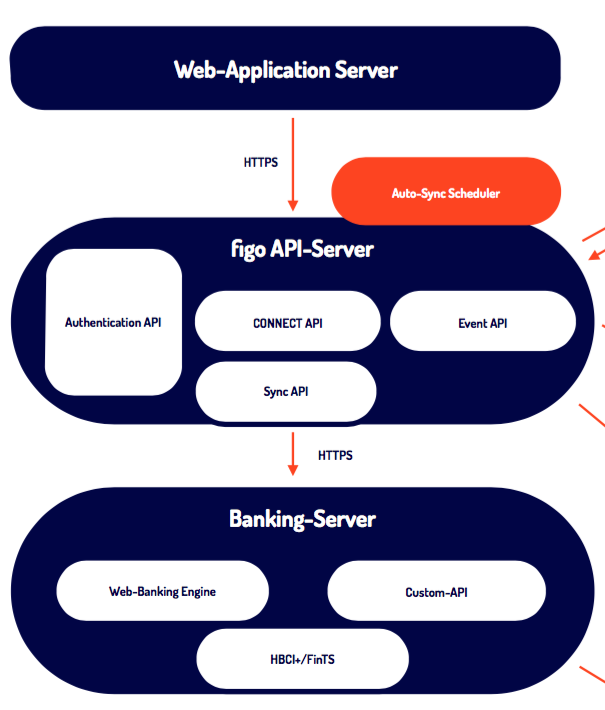
\includegraphics[scale=0.7]{grafiken/figoArch}
     \caption{figo GmbH high level architecture}
\end{figure}

\subsection{Banking Server Architecture}
\label{sec:bankingArch}
	Banking server has three parts for communication with banks via three separate channels. Each of them is a realization of different technology in a same programming language - javascript.  

	\paragraph{Custom-API} is responsible for connection to custom APIs provided by banks. It implements the client for custom banks APIs. Some of them provide full functionality while some only partial. All this APIs vary in their structure and functionality but most of them  are an implementation of REST-API specification.
	
	\paragraph{HBCI+/FinTS} is responsible for connection to banks' interfaces via Home Banking Computer Interface (HBCI). It is an implementation of an \textit{adapter OOP pattern} for the jsHBCI library.  HBCI is an open publicly available protocol. Its specification was originally designed by the two German banking groups \textit{Sparkasse and Volksbanken und Raiffeisenbanken} and \textit{German higher-level associations as the Bundesverband deutscher Banken e.V.}.  \cite{finTS}
	
	\paragraph{Web-Banking Engine} is responsible for communication with banks which does not provide API or HBCI. This is an implementation of a \textit{factory OOP pattern} for scraping libraries. Here figo GmbH uses \textit{web scraping} technology to perform interaction with internet-banking web pages.
	From the banks perspective, the interaction looks completely like direct communication with an user, while a user does not feel the difference between interaction via Custom-API or HBCI or Web-Banking Engine while accessing his bank or service via figo API.
	This is the most sensitive part from the developer's perspective since every change to the bank's web page can lead to failure of the specific scripts. \\
	
%	The aim of this paper is an application of Test Sheet for early (before any user's interaction will take place) recognition of page changes  and notification of developers regarding failed part of the script.
	
	%\subsection{Banking Technology Stack}
	%banking server only
	
%and analyses the difference in requirements differences defined by Test Sheets concept and introduced by figo GmbH.

%Firstly the platform of the implementation must be node.js its conceptual differences with such enterprise languages as Java or C# can be understood from the paltform description provided earlier in this paper but it worth to highlight them explicitly. The language of implementation is javascript which is the language with \textit{prototype based inheritance}. The \textit{event-loop mechanism} placed in core of the platform makes it asynchronous. Support of f\textit{unctions as a first-class citizens} provides an ability of confrontational function passing which is a pattern of functional programming. The language is relatively new for implementation of server-side applications.



%Test Sheets were originally designed for test definitions of OOP languages. And all available examples describes tests definitions for Java Classes. While figo GmbH case requires implementation of tests for nodeJS/casperJS, which are based on JavaScript - Object Oriented, imperative, Functional Oriented programming language with asynchronous information flow.
%Moreover figo GmbH requires input of test results to be recorded in to LogStash logs database. 

%Testing of real-time software


%The execution requirements from figo GmbH are such that tests defined via Test Sheets should be automatically executed in a time manner (every 2 mins or so), while normal software testing is performed on demand.
%The figo's requirement for comparison is such that while defining a Test Sheet user should be able to select from two types of comparison: 1) Strict comparison - complete comparison of objects including both properties' structure and their values. 2) Not-Strict comparison - scheme comparison of objects.

%(Probably should go to different section)
%Scraping scripts implement callback based approach for handling asynchronous data flow. This provides an opportunity to perform result comparison within the custom callback defined on a implementation stage.
%Standard convention for callback definitions limitates number of input parameters of a callback (error, data), while comparison requires compare data parameter with expected outputs from Test Sheet. The opportunity to resolve this issue lays in a JavaScript's support of functions as a class citizens, the function implementation of module for comparison and report: module exports function which invoked with single parameters (expected\_output) / ( + script name) and returns function which is used as a callback for scrapping script, this callback function performs comparison and writes its result to TestSheet or logstash depending on environment in which the program was executed


%%!!! update conventions and align this list to them!
%\begin{enumerate}
%	\item asynchronous software in combination with reference mechanism of test sheets
%\end{enumerate}

\section{Transformation project}
\label{sec:transP}
This section describes transformation project created by figo GmbH for use of Test Sheets within the organization.
\textbf{Enterprise System Transformation} -  "is a hierarchic-sequential process involving all actions of individuals in an organization leveraging information technology to support the transition of an Enterprise System from its original O-I-T[(Fir.:\ref{fig:oit})] configuration [...] to an (enhanced) O-I-T[(Fir.:\ref{fig:oit})] configuration."\cite{MES5}

\begin{figure}[ht]
	\label{fig:oit}
	\centering
	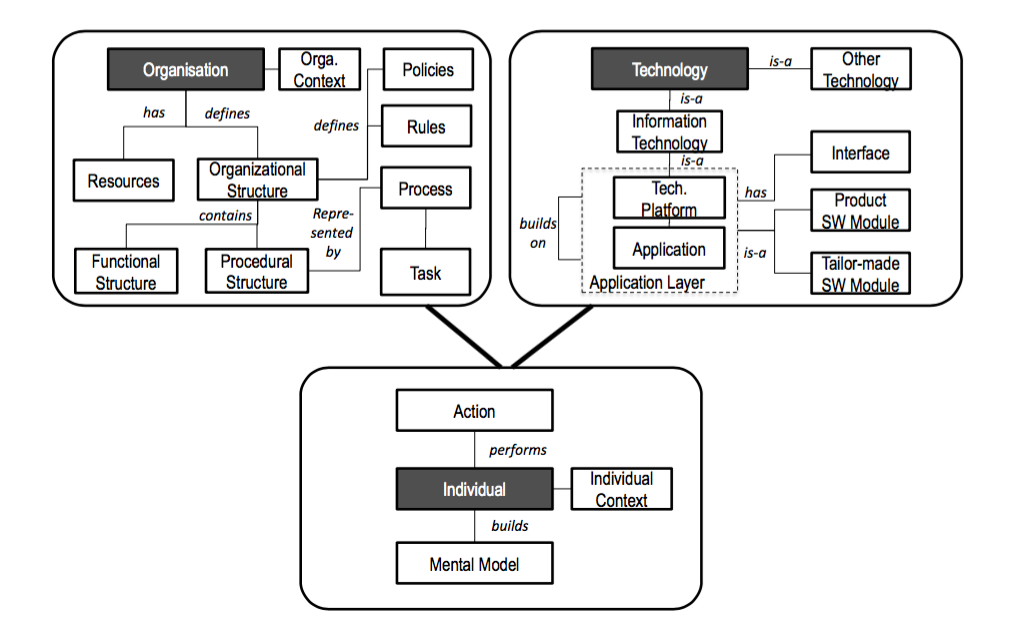
\includegraphics[width=\textwidth]{grafiken/oit.png}
	\caption{O-I-T model\cite{MES5}}
\end{figure}

The transformation project includes within itself four processes:
\paragraph{Development} focuses on the issue how information systems are developed. In contrast to software engineering, software development takes the socio-technical perspective on information systems\cite{MES6}.

\paragraph{Adoption} is a process defined by three concepts\cite{MES7}
\begin{enumerate}
	\item \textbf{Diffusion} refers to the breadth of use, e.g.the number of adopters in an organization
	\item \textbf{Infusion} describes how extensively the technology is used and the level of impact within the organization
	\item \textbf{Assimilation} addresses how extensively the new technology is used and how deeply the firm's use of the technology alters processes, structures, and organizational culture
\end{enumerate}

\paragraph{Convertion} is a process of realization of transformation projects with goal of successful system transformations \cite{MES9}

\paragraph{Use} continues process closely coupled with conversion process. It covers not only the process of the system usage by the individuals but also the impact of it on the organization in context of short- and long-term benefits. Individuals in the context of their performance and satisfaction.

\subsection{Test Sheets project}



%The tool should provide business staff of the company to define business scenarios in a non-technical way. After definition such scenarios must be executed over web-page. Create, Read, Update, Delete (CRUD) operations for this scenarios must be performed with .

\paragraph{Project definition:} Introduction of a tool for verification and/or testing of product’s functional fit to its requirements (i. e. detection of changes in banks web-pages, local software failures and/or errors) with minimal involvement of software developers into the process. Continuous project which requires software to be developed and supported by developers and can be executed on workstations of product/project managers.

\paragraph{Project uncertainties.}
\begin{itemize}
	\item Priority
	\item Functional fit
	\item Maintenance process
	\item Usage enhancement
	\item Organizational culture fit
\end{itemize}

\paragraph{Rationale for project creation and focus.} High load on developers caused by requirements to the speed of delivery reduced amount of time available for system monitoring. Repairment time estimation required by customers user experience. 


\paragraph{Underlying assumptions.} Shift of responsibility for functionality  on managers will improve system maintenance process and customers' user experience. 

\paragraph{Goal.} Routinization of product verification/testing process with respect to its business and functionality requirements by use of Test Sheets.
\paragraph{Plan:}
\begin{itemize}
	\item Test Sheets introduction to the target customers
	\item Requirements analysis 
	\item Mapping requirements to the concept of Test Sheets
	\item Development process definition
	\item System design
	\item Development
	\begin{itemize}
		\item Alpha1 version without support of references and optimization for real-time testing
		\item Alpha2 version with references support and optimization for real-time testing
		\item BETA version with optimization for real-time testing
		\item Reporting mechanism
	\end{itemize}
	\item Introduction (demonstration)
	\item Learning
	\item Routinization
\end{itemize}

\paragraph{Success.} Goals are met, system is fully routinized within the business processes, time for bugs allocation and fix is reduced. The number of affected customers is minimized.


\subsection{Technical requirements}
First, test execution must be performed in a timely fashion for an opportunity to detect changes as early as possible to prevent attempts of customers' communication with not available banks or services. Consequently, tests execution have to be fast. 
Nextm software developers must be notified about script failure as soon as it was detected to improve response time. 
Moreover, scraping scripts are communicating with web-pages in a real-time and asynchronous fashion. 
Further, the language of implementation must be javascript for low entry level of developers in the future maintenance process. 
Last but not least, due to the nature of data represented on a web page the comparison between actual and expected results must have two possible options: object keys comparison and object key-value comparison.



\chapter{Software testing}
\label{chap:testing}
%Oxford dictionary defines test as a procedure intended to establish the quality, performance, or reliability of something, especially before it is taken into widespread use. 
Software testing is an important technique to evaluate and assess software's quality and reliability, it provides possibility to determine whether the development of product conform the requirements. The variety of tests coincides the variety of requirements for the software under test. At least 30\% of the price of a software project is the cost of software testing \cite{Lecture2}. 
The general requirements to test definitions are following: fast, independent, repeatable, self-validating, timely.
More detailed information regarding requirements can be found via following URL: \url{http://www.extremeprogramming.org/rules/testfirst.html}
 %The price of software project for at least 30\% consists of costs for tests\cite{Lecture2}.
%The knowledge on software testing have become crucial for all software developers and engineers\cite{IntroductionST}.
%Robert Cecil Martin in his book 'Clean Code: A Handbook of Agile Software Craftsmanship'\cite{MartinClean} says following: "Tests are as important to the health of a project as the production code is. Perhaps they are even more important, because tests preserve and enhance the flexibility, maintainability, and reusability of the production code."
%"Test processes determine whether the development products of a given activity conform to the requirements of that activity and whether the system and/or software satisfies its intended use and user needs. Testing process tasks are specified for different integrity levels. These process tasks determine the appropriate breadth and depth of test documentation. The documentation elements for each type of test documentation can then be selected. The scope of testing encompasses software-based systems, computer software, hardware and their interfaces. This standard applies to software-based systems being developed, maintained, or reused (legacy, COTS, Non-Developmental Items). The term software also includes firmware, microcode and documentation. Test processes can include inspection, analysis, demonstration, verification and validation of software products."\cite{draft}
\paragraph{The economic costs} of unexpected software behavior (bug, failure or error) can go up to several millions or even billions of USD. \\
\textit{\textbf{Web application failures}} only in the USA lead to losses of \$6.5 million per hour in financial services and \$2.4 million per hour in credit card sales applications\cite{Lecture1}. \\
\textit{\textbf{Alarm-management}} fault was one of the reasons of the black-out occurred in the northeastern US on August 2003. Estimated costs were between US\$7 and \$10 billion\cite{costOfErrors}.\\
\textit{\textbf{In general,}} according to report made by US National Institute of Standards and Technology (NIST) in 2009 the estimated economy loses  were \$60 billion annually as associated with developing and distributing software patches and reinstalling systems that have been involved, together with losses in productivity due to errors and malware infections\cite{costOfErrors}.\\


\paragraph{The human causalities} caused by software misbehavior can rich dramatic scales.\\
\textit{\textbf{The case of Toyota}} unintended acceleration caused by software defect  in 2009 - 2011 led to 89 deaths and 57 injures.
Toyota was fined \$1.2 Billion for concealing safety defects\cite{toyota}.\\
\textit{\textbf{The Patriot,}} surface-to-air missile, system failed to track and intercept an incoming Scud missile on 25 of February 1991. As the result 28 soldiers were killed and around 100 were injured\cite{costOfErrors}.\\
\textit{\textbf{A Therac-25}}, linear accelerator, which failure caused to 6 know cases where cancer patients received deadly radiation overdoses during their treatment between June 1985 and January 1987. The dosages were 100 times exceeding typically used for treatment\cite{costOfErrors}\cite{therac}.\\

%The variety of tests coincides the variety of requirements for the software under test. Test processes determine whether the software conform to the requirements and/or satisfies its intended use and user needs\cite{ieeeTesting}. As well as this is an important technique to evaluate and help to improve software quality, reliability and saftiness\cite{cota}.





%This led to new requirements for testing definition and representation tools since old tools like JUnit have high entry level for test engineers and requires its users to have an ability to write and read an executable code in a corresponding programming language.




%According to IEEE Standard for Software and System Test Documentation the process of software testing includes "inspection, analysis, demonstration, verification, and validation".

%"Test processes determine whether the development products of a given activity conform to the requirements of that activity and whether the system and/or software satisfies its intended use and user needs. Testing process tasks are specified for different integrity levels. These process tasks determine the appropriate breadth and depth of test documentation. The documentation elements for each type of test documentation can then be selected. The scope of testing encompasses software-based systems, computer software, hardware, and their interfaces. This standard applies to software-based systems being developed, maintained, or reused (legacy, commercial off-the-shelf, Non-Developmental Items). The term "software" also includes firmware, microcode, and documentation. Test processes can include inspection, analysis, demonstration, verification, and validation of software and software-based system products."\cite{ieeeTesting}


%"Software testing has grown as an important technique to evaluate and help to improve software quality.
%Numerous techniques and tools have appeared in the last decade, ranging from static analysis to automatic test generation and application.
%One can argue that software is the dominant part of an embedded system, either as a final product (executable code) or during its development lifecycle (system modeling in specific languages and computation models).
%In both cases, software must be thoroughly verified to ensure product quality and reliability.
%One can observe a growing number of academic and industrial works on the topic of embedded SW testing in the last four or five years, and this seems to be a good time for reflection: how exactly is embedded software testing different from traditional software testing? 
%Is it an engineering or computer science problem? 
%Does it need extra support from platform developers? 
%What is the role of the SW engineer and of the designer in developing a high-quality software-based embedded application?
%Many authors suggest that, on top of the ordinary software testing challenges, software usage in an embedded application brings additional issues that must be dealt with: the variety of possible target platforms, the different computational models involved during the design, faster time-to-market and even more instable and complex specifications, platform-dependent constraints (power, memory, and resources availability), etc.
%On the other hand, current platforms are more and more powerful, and the specificities of the embedded application can help to reduce the search space during test generation:
%application domains, strong code reuse paradigm, use of less advanced programming language resources, and common availability of system models subject to or already verified with respect to specific properties, for instance.
%Furthermore, a major part of the so-called embedded software does not depend directly on hardware, and one can argue that only a small percentage really needs to be tested together with the target platform, and this test is part of the platform design, not the system design. "\cite{cota}

%Introduction of Agile and Extreme development paradigms with increased requirements for control over the existing code, its reuse and maintenance lifted requirements for tests and their quality to the new level and shifted responsibility regarding testing process from software engineers to people without development background. 
%This led to new requirements for testing definition and representation tools since old tools like JUnit have high entry level for test engineers and requires its users to have an ability to write and read an executable code in a corresponding programming language.

\section{Existing approaches for test definitions}
\label{sec:testApproaches}
In most of the cases developers are using testing frameworks or internal DSLs which requires the use of formal programming languages. This, in a result, makes writing of tests not different from the programming. It requires knowledge of languages and understanding of the basic programming concepts from everyone who is involved in the creation of a test, reading its result or updating/deleting the test.
%Since it is common practice to base tests on top of business requirements tests should be used by different shareholders who define those requirements.
The brief overview of different testing approaches and their analysis with respect to modern business requirements is provided below.

\subsection{xUnit}
xUnit is a family of unit testing frameworks with shared architecture and functionality which is derived from Smalltalk's SUnit, designed for tests automation\cite{xunit}\cite{xunitFowler}. The general simplicity and lightweight made them as a popular tool for Test Driven Development\cite{xunitFowler}.

xUnit basic features implemented by all members of the family provide functionality to perform following tasks\cite{xunit}:
\begin{enumerate}
	\item Specify a test as a \textit{Test Method};
	\item Specify the expected results within the test method in the form of calls to \textit{Assertion Methods};
	\item Aggregate the tests into test suites that can be run as a single operation;
	\item Run one or more tests to get a report on the results of the test run
\end{enumerate}

Test \textbf{\textit{cases}} in xUnit are defined as a methods united in to \textbf{\textit{suites}} with shared preconditions called \textbf{\textit{fixtures}}.  Cases or suites are executed by a \textbf{\textit{runner}} which compares actual and expected results using \textbf{\textit{assertion}} function.

The family includes a wide variety of implementations for multiple programming languages, and diverse enhancement of functionality (e. g. code coverage statistics, assertion add-ons etc.)\cite{xunitWiki}.

Definition of tests with formal general programming language from one side makes tests definition and execution fast but at the same time makes impossible the creation of tests for people without developer background. 

\subsection{Fit}
Framework for Integrated Test (Fit) - is a way of defining test cases with HTML pages. It enhances the communication and collaboration connecting customers and programmers. Moreover, it creates a feedback loop between them. Fit automatically checks HTML pages against actual program\cite{fit}.

Fit reads tables in HTML files, each table is interpreted by a \textit{fixture} written by programmers. This fixture checks the examples in the table by running the actual program\cite{fitIntro}.

Programmers use a \textit{ColumnFixture} to map the columns in the table to variables and methods in the fixture. The first columns provide correspondence to variables in the fixture. The last column has the expected result and corresponds to the method in the fixture\cite{fitIntro}.

Different implementations provide different user experience from Wiki pages (i.e. FitNess) to complete standalone application with internal functionality for tables definitions and tests execution (i.e. GuiRunner).

With Fit, customers can provide more guidance in a development process by lending their subject matter expertise and imagination to the effort\cite{fit} requiring developer to write only \textit{fixture}, the middleware between tests and code. At the same time, it provides media between  CRUD operations over tests and the results of their execution for people without development experience.

\subsection{Cucumber}
Cucumber is a Behavior Driven Development tool which allows users to define tests specifications with \textit{Gherkin}, the language which is structured plain text with support of internationalization for 60+ different languages\cite{cuceRef}.

Feature files written in Gherkin consist of plain text and general key-words are used for identification of following concepts:
\begin{itemize}
	\item Feature under the test: \textit{Feature};
	\item Test scenario: \textit{Scenario};
	\item Scenario Outline: \textit{Scenario Outline}
	\item Test Steps: \textit{Given, When, Then, And, But};
	\item Test Background:  \textit{Background};
	\item Test Examples: \textit{Examples}
\end{itemize}

Specific characters are used for identification of:
\begin{itemize}
	\item Step Inputs: String - \textit{"""}, Table - \textit{$|$};
	\item Step Tags: \textit{@};
	\item Comments: \textit{\#}
\end{itemize}

Step definitions are written by developers. Definition parses feature file with attached pattern to link all the step matches and code executed by cucumber when match is met.

Human readable input and output of the tests defined in gherkin makes cucumber a good media for communication between people who create requirements and those who are trying to meet them. But at the same time software development experience required for writing code with step definitions.

\section{Test Sheets}
\label{sec:testSheets}
Test Sheets is a representation for tests developed with the goal to combine the power and completeness of formal programming language with a representation that is easy to understand and work with even for people with little IT knowledge\cite{ts}.

Test Sheets approach uses a usual spreadsheet for a definition of test and representation of their result. 
\begin{itemize}
	\item Rows - represent operations being executed;
	\item Columns -  variables for input or output parameters;
\end{itemize}

The actual content of a cell can be made dependent on other cells by addressing them via their location.
Just like in Fit, the result of tests execution is provided in the same table with coloring and actual return are separated by "\textbackslash"\ symbol in case of failing test\cite{tsb}.

There are three types of test sheets which can be used in combination:
\begin{itemize}
	\item \textbf{Basic} - order of test step execution is defined by order of rows in a table;
	\item \textbf{Non-Linear} - order of test steps execution is defined by finite state machine with states represented by test steps and transition function by step execution results or number of test step execution;
	\item \textbf{High-Order/Parametrized} - The actual value used for Parameterized Test Sheets is specified by a Higher-Order Test Sheet in a column with letter Parametrized Test Sheet refers to.
\end{itemize}
The main benefit of this approach over \textit{xUnit}, \textit{Cucumber}, \textit{Fit} is an exclusion of software developers from tests definitions which can be performed by a user without prior development experience with usage of any spreadsheet editor.

 \subsection{Basic Test Sheets}
A Basic Test Sheet is a type of Test Sheets with sequential tests execution without parametrized values, but with the possibility to use references between cells for definition of values.
The rows content is structured as following:
\begin{itemize}
	\item \textit{Test name} - first row;
	\item \textit{Class/Module under test} - second row;
	\item \textit{Test step} - all next rows represent method calls;
\end{itemize}

The values in columns cells which belong to the test step has net purposes:
\begin{itemize}
	\item \textit{Object Under Test} - cells in a first column;
	\item \textit{Method Under Test} - cells in a second column;
	\item \textit{Input Parameters} - cells in a next column before invocation line;
	\item \textit{Invocation Line} - cells in a delimiter column between cell(s) with biggest number of input and column with expected return value;
	\item \textit{Expected Return} - cells in a column after invocation line;
\end{itemize}

The description provided above is shown in a summarized example from the web site of Chair of Software Engineering of University of Mannheim (Pic.: \ref{fig:BasictestSheet}).
  \begin{figure}[ht]
  	\label{fig:BasictestSheet}
    \centering
    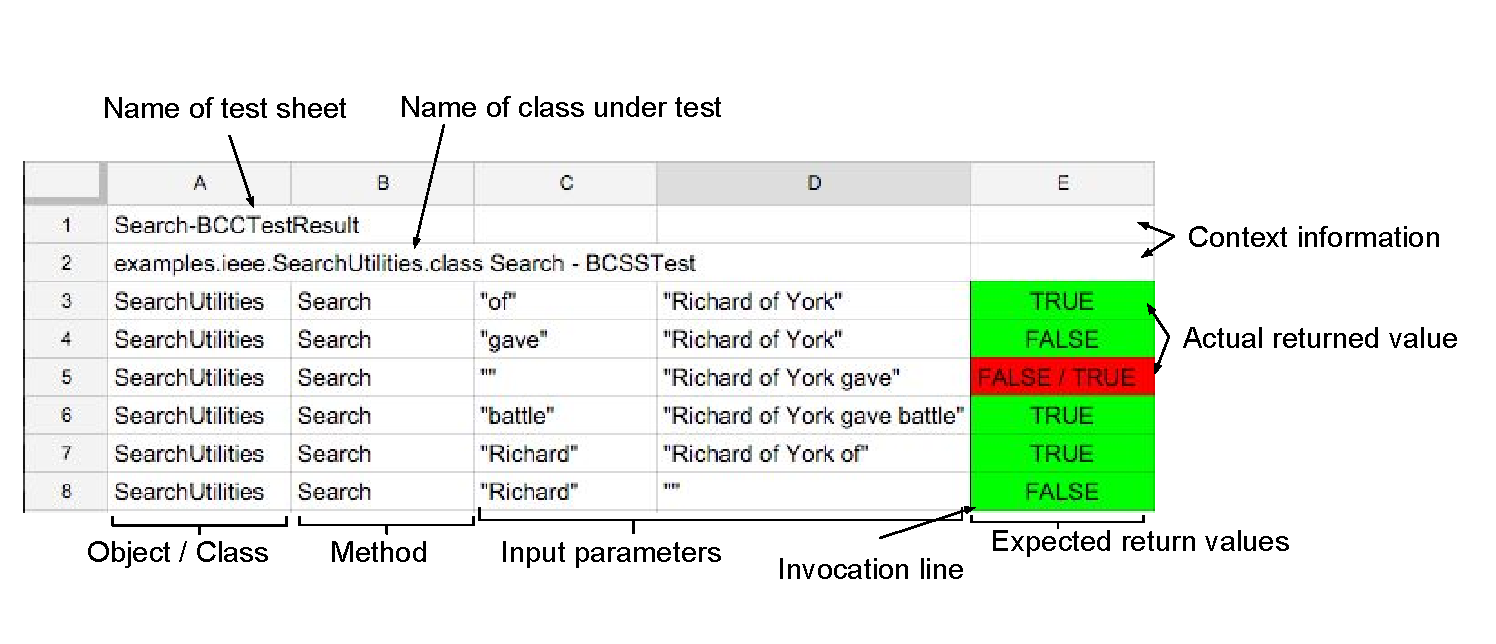
\includegraphics[width=\textwidth]{grafiken/basic_test_sheet}
     \caption{Basic Test Sheet}
  \end{figure}



The software developed within the scope of this research is a proof of concept for the usage of Test Sheets for scenario testing of asynchronous real-time software. The scope of this paper covers only Basic Test Sheets. For more details about Test Sheets and Research Topics of the Chair of Software Engineering please visit \url{http://swt.informatik.uni-mannheim.de/de/home/}.

% \paragraph{Non-Linear}
%Similar to the invocation line (double line separating input parameters and expected return values) there is a double line below the last method invocation row.
%Below this line the behavior specification starts. 
%Each row of the behavior specification represents a state of a state machine. 
%The state machine starts in the first state that is being specified right below the double line and stops execution once a state is reached without any valid transitions.

%Each column in a row specifies a transition. 
%A transition consists of a guard, executed invocations and a subsequent state. 
%The starting state has only one transition with no guard, the intermediate state has [...] transitions each with a guard and the terminating state does not have any transitions at all[...].  \cite{tsn}

%\section{High Order, Parameterized Test Sheets}
%"The actual value used for Parameterized Test Sheets is specified by a Higher-Order Test Sheet as in the example below. 
%The Higher-Order Test Sheet references the Parameterized Test Sheet as the 'class' being tested. 
%On said pseudo-class it invokes the pseudo-method test followed the by the value to be used as parameter. 
%?C in the Parameterized Test Sheet is replaced by the value defined the third column (column C) for each execution.
%It is also possible to use more than one parameter. These are defined in the Higher-Order Test Sheet in subsequent columns (D, E, F, etc.) and referenced in the Parameterized Test Sheet via ?D, ?E, ?F, etc"\cite{tsh}

\chapter{Real-Time Software and its Testing. Web scrapping}
\label{chap:rt}
\section{Real-Time Software}
Donald Gillies defined a real-time software as a system: \textit{"[...] in which the correctness of the computations not only depends upon the logical correctness of the computation but also upon the time at which the result is produced. If the timing constraints of the system are not met, system failure is said to have occurred."} While Robert L. Glass\cite{RealTimeTesting} defines this term as: \textit{"[...] a software that drives a computer which interacts with functioning external devices or objects. It is called real-time because the software actions control activities that are occurring in an ongoing process".} 

Within this research, we will define  \textit{Real-Time software} as a combination of this to definitions which covers both logical and time correctness as well as an interaction with external systems controlled by the ongoing process.

The Web-Banking engine of figo GmbH matches this definition due to the following facts. First, it performs communication with external systems (Web Banking HTML pages). Next, its result correctness depends on time restrictions (if child process responsible for script execution was not finished within 1200 seconds, and with each task performed within 0.5 seconds it is treated as failed) as well as logical correctness depended upon ability of the script to perform necessary actions for a fulfillment of a requested task.

%Within the scope of this research under Real-Time software we will mean the software that interact with external systems and its correctness depends on logical correctness of execution result as well as result production time.

%Not only do the programmers have to look at black/white box testing but also the timing of the data \& the parallelism of the projects. In lots of situations testing data for real-time technique may raise errors when the technique is in four state but to in others.\cite{strategicRT}

%"During the development of a real-time application, a testing step is necessary to check the conformity of the implementation in accordance with its specification. "\cite{trts}

%In general the special characteristic of real-time systems makes them a main challenge when it comes to testing. The time-dependent type of real-time applications adds a new difficult element to testing.

\section{Testing Real-Time software}
Tsai, Fang and Bi\cite{rtSandD} state that testing and debugging of real-time software are very difficult because of timing constraints and non-deterministic execution behavior. In a real-time system, the processes receive inputs from real world processes as a result of asynchronous interrupts and it is almost impossible to precisely predict the exact program execution points at which the inputs will be supplied to the system. Consequently, the system may not exhibit the same behavior upon repeated execution of the program. In addition, in a real-time system, the pace of an execution of processes is determined not only by internal criteria but also by real world processes and their timing constraints. 

The general testing and debugging strategy (Fig. \ref{fig:GeneralTestingAndDebugging}) described by Tsai, Fang and Bi \cite{rtSandD} consists of four steps.
At the \textit{first} step, a set of events which can be used to represent the program's execution behavior at a specific abstraction level and the event key values which describe these events are identified. 
At the \textit{second} step, the execution data, containing the event key values identified in the fist step, is collected using the real-time monitoring system. 
The first and second steps constitute the monitoring phase. After the data is collected, at the \textit{third} step, the collected data is processed in an off-line mode to construct logical views to represent the program's execution behavior.
At the \textit{fourth} step, analysis algorithms will be employed to identify fault units and to report to the user. 
Finally, the user can use this report to decide next monitoring and debugging cycle for a lower level abstraction.
In this paper, the provided strategy is applied for each individual test.

\begin{figure}[ht]
	\centering
	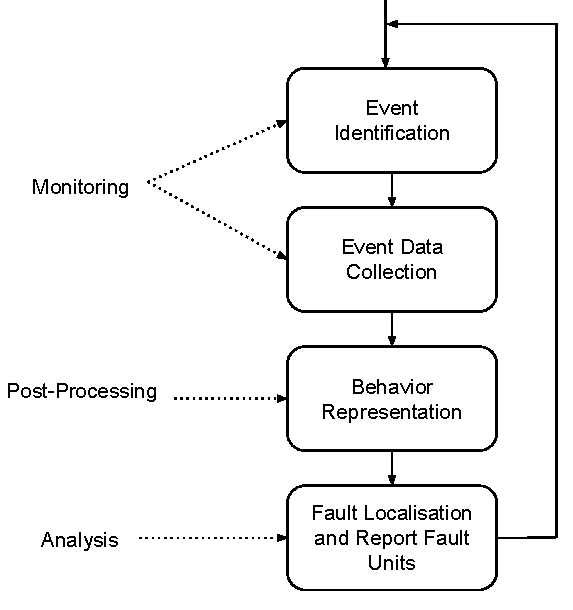
\includegraphics[width=0.7\linewidth]{grafiken/GeneralTestingAndDebugging}
	\label{fig:GeneralTestingAndDebugging}
	\caption{General Testing and Debugging Strategy\cite{rtSandD}}
\end{figure}

\section{Web scraping. CasperJS}
\label{sec:scraping}
Web scraping is a method for extracting information from web pages\cite{wikiScraping}. This technique is useful when you want to do real-time, price and product comparisons, archive web pages, or acquire data sets that you want to evaluate or filter\cite{conScrap}.

Web scraping works via interaction with Document Object Model (DOM) of the web page it is a useful technique for real-time data extraction from human readable web-pages. W3Council defines DOM\cite{w3cDOM} as "... a platform- and language-neutral interface that will allow programs and scripts to dynamically access and update the content, structure and style of documents." 

\paragraph{CasperJS} is an open source navigation scripting \& testing utility written in javascript for the headless browsing. It eases the process of defining a full navigation scenario and provides useful high-level functions, methods \& syntactic sugar for doing common tasks for interaction with DOM of the web page\cite{casperjs}:
\begin{itemize}
	\item defining \& ordering browsing navigation steps
	\item filling \& submitting forms
	\item clicking \& following links
	\item capturing screenshots of a page (or part of it)
	\item testing remote DOM
	\item logging events
	\item downloading resources, including binary ones
	\item writing functional test suites, saving results as JUnit XML
	\item scraping Web contents
\end{itemize}

Usage of this tool gives an ability for figo GmbH to pragmatically imitate user behavior on a web page. Which includes filling login forms, filing forms for retrieving service information and perform other business activity available via a service web site. CasperJS instantiates web-page or its part defined as tree of DOM selectors.  Page content includes both HTML and javascript/jQuery code from the web-page addressed with provided URL. Instantiated page or its part is stored in memory and can be accessed for further manipulation by CasperJS methods as any other object instance.
 \chapter{Asynchronous programming. Strategies and performance}
 \label{chap:async}
\section{Asynchronous programming}
\label{sec:async}
Asynchronous programming is the programming model in which operations should be done are interleaved with one another within the single control thread. An analogy to it can be package multiplexing in a Computer Networks. 

To compare to multi-threaded systems are synchronous and allow execution of one task per unit of time blocking execution of other tasks until programmer will perform explicit control delegation to another task.

Generally, asynchronous systems are easier to control and to develop rather then multi-threaded, and  they perform better then synchronous in following cases\cite{asyncArticle}:
 \begin{itemize}
	\item Large number of tasks and, at least, one task likely to make progress;
	\item A lot of I/O operations;
	\item Tasks are independent of one another;
 \end{itemize}



\subsection{node.js}
\label{subsec:node}
node.js is an asynchronous event-driven framework designed to build scalable network applications.
node.js is similar in design to and influenced by systems like Ruby's Event Machine or Python's Twisted with the difference that it presents the event loop as a language construct instead of as a library\cite{nodejsabout}.

node.js as a framework has powerful ecosystem - npm which consists of three parts. \textit{npm} - package manager for node.js, \textit{npm Registry} - public collection of packages of open-source code, \textit{npm command line client} which allows developers to install and publish those packages. On a diagram (Fig.: \ref{fig:npmStat}) stated the comparison of npm with other package managers made by module counts, for more up to date information please visit \url{http://www.modulecounts.com/}.
\begin{figure}[ht]
	\label{fig:npmStat}
	\centering
	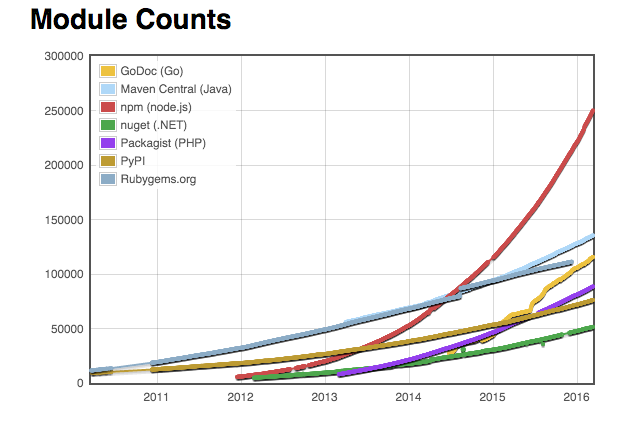
\includegraphics[width=\textwidth]{grafiken/modulecounts.png}
	\caption{npm comparison with other package managers\cite{moduleCounts}}
\end{figure}

At the same time there is a downside of such ecosystem. The case of \textit{left-pad} the module which was deleted from the npm due to copyright concerns caused by the failure during the build process for thousands of projects\cite{npmDown}. Further, there are three factors explained by Sam Saccone \cite{npmHydra} \cite{npmSoft} which make npm a root source of hackers attack since all life-cycle scripts executed by installed packages are executed with same privilege level as user invoked their installation. The \textit{first} reason is caused by the usage of SemVer for version controlling which does not lock dependencies to a specific version The\textit{ second }reason is the lack of automatic npm user log-out.  Since npm can run arbitrary scripts on install that means that any user who is currently logged in and types npm install is allowing any module to execute arbitrary publish commands. The \textit{third} reason is dependent on that fact that a singular npm registry is used by the large majority of the node.js ecosystem on a daily basis.

General suggestions to overcome this problems for project developers and maintainers are following.
\begin{itemize}
	\item disable life-cycle scripts during update/install process;
	\item lock down all dependencies versions either manually or using shrinkwrap package \url{https://docs.npmjs.com/cli/shrinkwrap}
	\item sotre dependencies locally and use them as a part of source code being deployed.
\end{itemize}


Node.js applications are written in javascript - a lightweight dynamic scripting multi-paradigm language with first-class functions and prototype-based inheritance which provides both object-oriented and functional programming approaches\cite{mdnJS}.

When it comes to inheritance, JavaScript only has one construct: objects\cite{mdnProto}.
This can be called classless, prototype-oriented, or instance-based programming\cite{mdnOOP}. Each object has an internal link to another object called its \textit{prototype}. That prototype object has a prototype of its own, and so on until an object is reached with \textbf{null} as its prototype. \textbf{null}, by definition, has no prototype and acts as the final link in this prototype chain. JavaScript objects are dynamic "bags" of properties (referred to as own properties). When trying to access a property of an object, the property will not only be sought on the object but on the prototype of the object, the prototype of the prototype, and so on until either a property with a matching name is found or the end of the prototype chain is reached\cite{mdnProto} This type of inheritance provide objects inherit both instance and class methods and properties.

 
The high-level architecture of node.js looks following:(\ref{fig:nodeArch}). 
\begin{figure}[ht]
  	\label{fig:nodeArch}
    \centering
    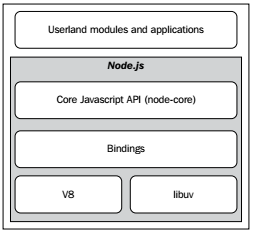
\includegraphics[scale=1.0]{grafiken/nodeArchitecture.png}
     \caption{Node.js architecture \cite{nodejsbook}}
  \end{figure}

\textit{Node core} is a javascript library (called node-core) that implements the high-level node.js API.

\textit{Bindings} responsible for wrapping and exposing \textit{libuv} and other low-level functionality to javascript.\cite{nodejsbook}

\textit{Non blocking I/O} provided by libuv\cite{nodejsabout}\cite{nodejsbook}. 
Which is "a multi-platform support library with a focus on asynchronous I/O. "\cite{libuv} with following properties\cite{libuvBasic}:
\begin{itemize}
\item Abstract operations, not events
\item Support different nonblocking I/O models
\item Focus on extendability and performance
\end{itemize}

\textit{V8/Chakra} the JavaScript engine originally developed by Google for the Chrome browser/ Microsoft for IE 9 browser"\cite{nodejsbook} 



\subsection{Event handling}
\label{subsec:event}
An event is a core concept of asynchronous programming in node.js. All objects that emit events allows one or more functions to be attached to named events emitted by the object. When an event is emitted all of the functions attached to that specific event are called synchronously\cite{events}. Node.js  event handler is an implementation of \textit{reactor pattern}. The illustration of process life-cycle is shown in Fig. \ref{fig:nodeEvent}:

\begin{figure}[ht]
  	\label{fig:nodeEvent}
    \centering
    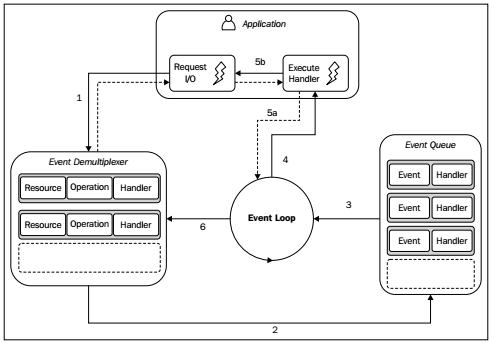
\includegraphics[width=\textwidth]{grafiken/nodeEventHandling.png}
     \caption{Node.js event handling system \cite{nodejsbook}}
  \end{figure}

\begin{enumerate}
	\item The application generates a new I/O operation by submitting a request to the \textit{Event Demultiplexer}. The application also specifies a \textit{listener}, which will be invoked when the operation completes. Submitting a new request to the Event Demultiplexer is a non-blocking call and it immediately returns the control back to the application.
	\item When a set of I/O operations completes, the Event Demultiplexer pushes the new events into the \textit{Event Queue}.
	\item At this point, the \textit{Event Loop} iterates over the items of the Event Queue.
	\item For each event, the associated listener is invoked.
	\item The listenr, which is part of the application code, will give back the control to the Event Loop when its execution completes. However, new asynchronous operations might be requested during the execution of the listener, causing new operations to be inserted in the Event Demultiplexer, before the control is given back to the Event Loop.
	\item When all the items in the Event Queue are processed, the loop will block again on the Event Demultiplexer which will then trigger another cycle.
\end{enumerate}

\section{Asynchronous handling strategies}
\label{sec:asyncstrat}
\subsection{Continuation passing}
The presence of functions as a first class citizens in javascript allows direct usage of functions for handling asynchronous program behavior. \textit{Callbacks} default are handlers for the reactor pattern described before. They are similar to \textit{visitor pattern} in OOP, they also represent an operation to be performed on the elements of an object structure and they let define a new operation without introducing any changes to the definition of the object. 

Callbacks implement continuation-passing-style from Functional Programming. By convention callbacks must be passed as the last argument and accept two parameters, the first is an error and the second is a data to be processed further.

There are two main negative sides of using callbacks. One of them is so-called \textit{callback hell} occurs due to the abundance of closures and in-place callback definitions. This makes the code hard to be read because of high level nesting, as well as written due to a scope of nesting and difficult to manage because of possible memory leaks created by closures. Another negative side is called \textit{releasing Zalgo}\cite{zalgo}, it occurs only in case of inconsistent function behavior when under some hidden conditions a function performs a synchronous action but some under other - asynchronous.

\subsection{Imperative}
Before starting with imperative strategies for handling of asynchronous data flow we would like to show the \textit{concept of duality} (Fig. \ref{fig:dualityMatrix}). showed by Erik Meijer \url{https://channel9.msdn.com/Events/Lang-NEXT/Lang-NEXT-2014/Keynote-Duality} and hardly used by Kris Koval in his \textit{General Theory of Reactivity} \url{https://github.com/kriskowal/gtor/}. This chapter is based on works of Kris Koval, Erik Meijer, Conal Eliot and Mark S. Miller in a field of Reactive Programming.

\begin{figure}[ht]
	\label{fig:dualityMatrix}
	\centering
	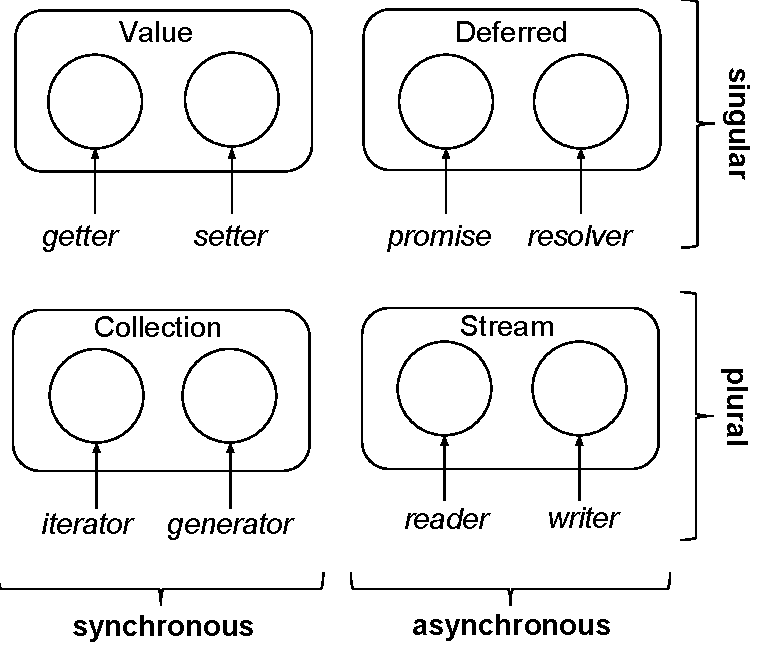
\includegraphics[scale = 0.5]{grafiken/dualityMatrix}
	\caption{Duality Matrix \cite{gtor}}
\end{figure}

The explanation of asynchronous patterns in this chapter will be performed via two-dimensional mapping. The first dimension is a time where things can be \textit{synchronous} and \textit{asynchronous}. Another dimension of space where mapping is done between \textit{singular} and \textit{plural}.

During communication can occur the problem caused by the fact that different parts for the dialog can have different load and different performance. The first situation is the \textbf{Fast producer - slow consumer} - the get of one entity works faster then the set of next entity in the chain. This situation occurs when values are \textbf{\textit{pushed}} by a producer. The second situation is the  \textbf{Slow producer - fast consumer} - thr get of one entity works slower then the  set of next entity in the chain. This situation occurs when values are \textbf{\textit{pulled}} by consumer. The solution of  this problems lays in a scope of the system design which should allocate push and pull entities in an appropriate sides of the communication channels.

\paragraph{Synchronous:} \textbf{Value} is a singular unit data. Its duals are \textit{getter (pull)} and \textit{setter (push)}. Setter accepts a value to be assigned and return nothing and getter accepts nothing and returns a value. The chaining process  can be performed here by applying setter to getter and getter to setter and by applying the same logic to their analogs for further  entities. A \textbf{Collection} is a plural form of the value. The duals of a collection are \textit{iterator (pull)} and \textit{generator (push)}. An \textit{iterator }as a plural analog of getter, it accepts nothing and returns the element from collection. A \textit{generator} is a plural analog of setter it accepts element to be added to collection and returns nothing.

\paragraph{Asynchronous:} \textbf{Deferred} is analog of the value. The duals for it are \textit{resolver (push)} and \textit{promise (pull)}. The resolver is an asynchronous analog of setter. It  accepts value which will be assigned as soon as it will be resolved. The promise is an asynchronous analog of the getter . It allows to obtain the value of the promise as soon as it will be resolved. The deferred concept guaranties unidirectional data flow which means that data can go only from resolver to promise. Further deferred entities guaranties asynchronism of execution for an operation which means they are "Zalgo safe"\cite{asyncPerformance}. \textbf{Stream} is an analog of the collection. It can be treated as a collection of deferred elements. The duals for stream are \textit{write (pull)} and \textit{read (push)}. The read is an analog of iterator it accepts nothing and takes values from the stream. The write is an analog of generator it accepts values from the stream and returns nothing. As a plural analog of deferred it guaranties unidirectional data flow.  The special case for streams in node.js are transform and duplex (transform) streams which are combination of read and write.


%\subsubsection{Streams}
%"A stream is an abstract interface implemented by various objects in Node.js." \cite{nodejsstreams}
%"Dominic Tarr (one of top contributors to the Node.js community \cite{nodejscontributors}), defines streams as node's best and most misunderstood idea."\cite{nodejsbook}

%Streams are the classic example of Pipe-and-filter architecture.

%"In an event-based platform such as Node.js, the most efficient way to handle I/O is in real time, consuming the input as soon as it is available and sending the output as soon as it is produced by the application."\cite{nodejsbook}

%\paragraph{Spatial efficiency.}
%"First of all, streams allow us to do things that would not be possible, by buffering data and processing it all at once. For example, consider the case in which we have to read a very big file, let's say, in the order of hundreds of megabytes or even gigabytes. 
%Clearly, using an API that returns a big buffer when the file is completely read, is not a good idea.
%Imagine reading a few of these big files concurrently; our application will easily run out of memory. Besides that, buffers in V8 (default NodeJS engine) cannot be bigger than 0x3FFFFFFF bytes (a little bit less than 1 GB). 
%So, we might hit a wall way before running out of physical memory." \cite{nodejsbook}

%\paragraph{Time efficiency.}
%"Let's now consider the case of an application that compresses a file and uploads it to a remote HTTP server, which in turn decompresses and saves it on the filesystem.
%If our client was implemented using a buffered API, the upload would start only when the entire file has been read and compressed. On the other hand, the decompression will start on the server only when all the data has been received. 
%A better solution to achieve the same result involves the use of streams. 
%On the client machine, streams allows you to compress and send the data chunks as soon as they are read from the filesystem, whereas, on the server, it allows you to decompress every chunk as soon as it is received from the remote peer."\cite{nodejsbook}

%\paragraph{Composability.}
%"The code we have seen so far has already given us an overview of how streams can be composed, thanks to the pipe() method, which allows us to connect the different processing units, each being responsible for one single functionality in perfect Node.js style. 
%This is possible because streams have a uniform interface, and they can understand each other in terms of API. The only prerequisite is that the next stream in the pipeline has to support the data type produced by the previous stream, which can be either binary, text, or even objects, as we will see later in the chapter.\\
%For these reasons, streams are often used not just to deal with pure I/O, but also as a means to simplify and modularize the code."\cite{nodejsbook}






\subsection{Performance}
\label{subsec:performance}
Following measures are taken from the article "Analysis of generators and other async patterns in node" by Gorgi Kosev (\url{https://spion.github.io/posts/analysis-generators-and-other-async-patterns-node.html}). There were no hardware characteristics provided for the experiment execution environment except following description\cite{asyncPerformance_2}: "On my machine redis can be queried about 40 000 times per second; node's 'hello world' http server can serve up to 10 000 requests per second; postgresql's pgbench can do 300 mixed or 15 000 select transactions per second." 

 The performance metrics were taken from the experiment under the the conditions where all external methods are mocked using setTimeout 10ms to simulate waiting for I/O with 1000 parallel requests (i.e. 100K IO / s) \cite{asyncPerformance_2}

\begin{table}[h]
	\begin{center}
		\begin{tabular}{| l | l | l | }
			\hline
			\textbf{pattern} & \textbf{time(ms)} & \textbf{memory (MB)} \\
			\hline
			promises-bluebird & 512 & 57,45 \\
			\hline
			promises-bluebird-generator & 364 & 41,89 \\
			\hline
			callbacks & 316 & 34.97 \\
			\hline
		\end{tabular}
	\end{center}
	\caption{Performance comparison of patterns for asynchronous information flow \cite{asyncPerformance_2}\cite{asyncPerformance}}
\end{table}


"The original and flattened solutions are the fastest, as they use vanilla callbacks"\cite{asyncPerformance}

Note that this table has only fastest among promise objects and since there were no measurements performed for streams but according to their nature the most optimistic performance for them should be equal to the promise generator provided by Bluebrid \url{http://bluebirdjs.com/docs/getting-started.html}.




%\chapter{OOP and FP}
\section{Object Oriented Programming}
"Programming languages with objects and classes typically provide dynamic lookup, abstraction, subtyping, and inheritance. These are the four main language concepts for object-oriented programming. They may be summarized in the following manner:
\textit{Dynamic lookup} means that when a message is sent to an object, the function code (or method) to be executed is determined by the way that the object is implemented, not some static property of the pointer or variable used to name the object. In other words, the object “chooses” how to respond to a message, and different objects may respond to the same message in different ways.
\textit{Abstraction} means that implementation details are hidden inside a program unit with a specific interface. For objects, the interface usually consists of a set of public functions (or public methods) that manipulate hidden data.
\textit{Subtyping} means that if some object a has all of the functionality of another object b, then we may use a in any context expecting b.
\textit{Inheritance} is the ability to reuse the definition of one kind of object to define another kind of object.
"\cite{concepts}

\subsection{Design Principles}

Agile design is a process, not an event.
It's the continous application of principles, patterns, and practices to improve the structure and readability of the software. 
It is the dedication to keep the design of the system as simple, clean, and expressive as possible at all times.\cite{MartinASD}

Symptoms of not agile design \cite{MartinASD}:
\begin{itemize}
	\item Rigidity - The design is difficult to change;
	\item Fragility - The design is easy to break;
	\item Immobility - The design is difficult to reuse;
	\item Viscosity - It is difficult to do the right thing;
	\item Needless complexity - Overdesign;
	\item Needless repetition - Mouse abuse;
	\item Opacity - Disorganized expression;
\end{itemize}
%\paragraph{Rigidity (The design is difficult to change)} - Rigidity is the tendency for software to be difficult to change, even in simple ways. A design is rigid if a single change causes a cascade of subsequent changes in dependent modules. The more modules that must be changed, the more rigid the design. Most developers have faced this situation in one way or another.  They are asked to make what appears to be a simple change. They look the change over and make a reasonable estimate of the work required. But later, as they work through the change, they find that there are unanticipated repercussions to the change. The developers find themselves chasing the change through huge portions of the code, modifying far more modules than they had first estimated, and discovering thread after thread of other changes that they must remember to make.In the end, the changes take far longer than the initial estimate.When asked why their estimate was so poor, they repeat the traditional software developers lament: "It was a lot more complicated than I thought!"

%\paragraph{Fragility (The design is easy to break)} - Fragility is the tendency of a program to break in many places when a single change is made. Often, the new problems are in areas that have no conceptual relationship with the area that was changed. Fixing those problems leads to even more problems, and the development team begins to resemble a dog chasing its tail. As the fragility of a module increases, the likelihood that a change will introduce unexpected problems approaches certainty. This seems absurd, but such modules are not at all uncommon. These are the modules that are continually in need of repair, the ones that are never off the bug list. These modules are the ones that the developers know need to be redesigned, but nobody wants to face the spectre of redesigning them. These modules are the ones that get worse the more you fix them.

%\paragraph{Immobility (The design is difficult to reuse)} - A design is immobile when it contains parts that could be useful in other systems, but the effort and risk involved with separating those parts from the original system are too great. This is an unfortunate but very common occurrence.

%\paragraph{Viscosity (It is difficult to do the right thing)} - Viscosity comes in two forms: viscosity of the software and viscosity of the environment. When faced with a change, developers usually find more than one way to make that change. Some of the ways preserve the design; others do not (i.e., they are hacks). When the design-preserving methods are more difficult to use than the hacks, the viscosity of the design is high. It is easy to do the wrong thing but difficult to do the right thing. We want to design our software such that the changes that preserve the design are easy to make. Viscosity of environment comes about when the development environment is slow and inefficient. For example, if compile times are very long, developers will be tempted to make changes that don't force large recompiles, even though those changes don't preserve the design.  If the source code control system requires hours to check in just a few files, developers will be tempted to make changes that require as few check-ins as possible, regardless of whether the design is preserved. In both cases, a viscous project is one in which the design of the software is difficult to preserve.  We want to create systems and project environments that make it easy to preserve and improve the design.


%\paragraph{Needless complexity (Overdesign)} - A design smells of needless complexity when it contains elements that aren't currently useful.This frequently happens when developers anticipate changes to the requirements and put facilities in the software to deal with those potential changes. At first, this may seem like a good thing to do. After all, preparing for future changes should keep our code flexible and prevent nightmarish changes later. Unfortunately, the effect is often just the opposite. By preparing for many contingencies, the design becomes littered with constructs that are never used. Some of those preparations may pay off, but many more do not.  Meanwhile, the design carries the weight of these unused design elements. This makes the software complex and difficult to understand.

%\paragraph{Needless repetition (Mouse abuse)} - Cut and paste may be useful text-editing operations, but they can be disastrous code-editing operations. All too often, software systems are built on dozens or hundreds of repeated code elements. It happens like this: Ralph needs to write some code that fravles the arvadent. He looks around in other parts of the code where he suspects other arvadent fravling has occurred and finds a suitable stretch of code. He cuts and pastes that code into his module and makes the suitable modifications. Unbeknownst to Ralph, the code he scraped up with his mouse was put there by Todd, who scraped it out of a module written by Lilly. Lilly was the first to fravle an arvadent, but she realized that fravling an arvadent was very similar to fravling a garnatosh.  She found some code somewhere that fravled a garnatosh, cut and paste it into her module, and modified it as necessary.When the same code appears over and over again, in slightly different forms, the developers are missing an abstraction. Finding all the repetition and eliminating it with an appropriate abstraction may not be high on their priority list, but it would go a long way toward making the system easier to understand and maintain. When there is redundant code in the system, the job of changing the system can become arduous. Bugs found in such a repeating unit have to be fixed in every repetition. However, since each repetition is slightly different from every other, the fix is not always the same.


%\paragraph{Opacity (Disorganized expression)} - Opacity is the tendency of a module to be difficult to understand. Code can be written in a clear and expressive manner, or it can be written in an opaque and convoluted manner. Code that evolves over time tends to become more and more opaque with age. A constant effort to keep the code clear and expressive is required in order to keep opacity to a minimum.When developers first write a module, the code may seem clear to them.After all, they have immersed themselves in it and understand it at an intimate level.Later, after the intimacy has worn off, they may return to that module and wonder how they could have written anything so awful. To prevent this, developers need to put themselves in their readers' shoes and make a concerted effort to refactor their code so that their readers can understand it. They also need to have their code reviewed by others.

Foundamental Object Oriented design principles\cite{Dooley}\cite{MartinASD} :
\begin{itemize}
 \item Closing - Encapsulate things in your design that are likely to change.
 \item Code to an Interface - rather then to an implementation. 
 \item Do not repeat yourself (DRY) - Avoid duplicate code.
 \item The Single-Responsibility Principle (SRP) - A class should have only one reason to change
 \item The Open/Closed Principle (OCP) - Software entities (classes, modules, functions, etc.) should be open for extension but closed for modification
 \item The Liskov Substitution Principle - Subtypes must be substitutable for their base types.
 \item The Dependency-Inversion Principle - A) High-level modules should not depend on low-level modules. 
Both should depend on abstractions. 
B) Abstractions should not depend upon details. 
Details should depend upon abstractions.
 \item The Interface Segregation Principle (ISP) - Clients should not be forced to depend on methods they do not use.
 \item Principles of Least Knowledge (PLK) - Talk to your immediate friends. 
 \item Principle of Loose Coupling - object that interact should be loosely coupled with well-defined intefaces.
\end{itemize}

%\paragraph{Closing} - Encapsulate things in your design that are likely to change. %This means to protect your classes from unnecessary change by separating the features and methods of a class that relatively constant throughout the program from that will change. By separating the two types of features, we isolate the parts that will change a lot into a separate class (or classes) that we can depend on changing, and we increase our flexibility and ease of change. \cite{Dooley}

%\paragraph{Code to an Interface} rather then to an implementation. \cite{Dooley}

%\paragraph{Do not repeat yourself (DRY)} - Avoid duplicate code. % Whenever you find common behaviour in two or more places, look to abstract tht behaviour into a class and then resue that behaviour in the common concrete classes. Satisfy one requirement in one place in your code\cite{Dooley}

%\paragraph{The Single-Responsibility Principle (SRP)} - A class should have only one reason to change.%In the context of the SRP, we define a responsibility to be a reason for change. If you can think of more than one motive for changing a class, that class has more than one responsibility. This is sometimes difficult to see. We are accustomed to thinking of responsibility in groups. The Single-Responsibility Principle is one of the simplest of the principles but one of the most difficult to get right. Conjoining responsibilities is something that we do naturally. Finding and separating those responsibilities is much of what software design is really about. Indeed, the rest of the principles we discuss come back to this issue in one way or another.\cite{MartinASD}\cite{Dooley}


%\paragraph{The Open/Closed Principle (OCP)} - Software entities (classes, modules, functions, etc.) should be open for extension but closed for modification.
%When a single change to a program results in a cascade of changes to dependent modules, the design smells of rigidity. OCP advises us to refactor the system so that further changes of that kind will not cause more modifications.  If OCP is applied well, further changes of that kind are achieved by adding new code, not by changing old code that already works.  This may seem like motherhood and apple piethe golden, unachievable idealbut in fact, there are some relatively simple and effective strategies for approaching that ideal. Modules that conform to OCP have two primary attributes. They are open for extension. This means that the behavior of the module can be extended. As the requirements of the application change, we can extend the module with new behaviors that satisfy those changes.  In other words, we are able to change what the module does. 1. They are closed for modification. Extending the behavior of a module does not result in changes to the source, or binary, code of the module. The binary executable version of the modulewhether in a linkable library, a DLL, or a .EXE fileremains untouched. 2. It would seem that these two attributes are at odds.  The normal way to extend the behavior of a module is to make changes to the source code of that module.  A module that cannot be changed is normally thought to have a fixed behavior.

%In many ways, the Open/Closed Principle is at the heart of object-oriented design.  Conformance to this principle is what yields the greatest benefits claimed for object-oriented technology: flexibility, reusability, and maintainability. Yet conformance to this principle is not achieved simply by using an object-oriented programming language. Nor is it a good idea to apply rampant abstraction to every part of the application.  Rather, it requires a dedication on the part of the developers to apply abstraction only to those parts of the program that exhibit frequent change. Resisting premature abstraction is as important as abstraction itself.\cite{MartinASD}\cite{Dooley}
%\paragraph{The Liskov Substitution Principle} - Subtypes must be substitutable for their base types.
%The Open/Closed Principle is at the heart of many of the claims made for object-oriented design. When this principle is in effect, applications are more maintainable, reusable, and robust.  The Liskov Substitution Principle is one of the prime enablers of OCP. The substitutability of subtypes allows a module, expressed in terms of a base type, to be extensible without modification. That substitutability must be something that developers can depend on implicitly. Thus, the contract of the base type has to be well and prominently understood, if not explicitly enforced, by the code. The term IS-A is too broad to act as a definition of a subtype.  The true definition of a subtype is substitutable, where substitutability is defined by either an explicit or implicit contract.\cite{MartinASD}\cite{Dooley}


%\paragraph{The Dependency-Inversion Principle} - A) High-level modules should not depend on low-level modules. 
%Both should depend on abstractions. 
%B) Abstractions should not depend upon details. 
%Details should depend upon abstractions.

%Consider the implications of high-level modules that depend on low-level modules.  It is the high-level modules that contain the important policy decisions and business models of an application. These modules contain the identity of the application.  Yet when these modules depend on the lower-level modules, changes to the lower-level modules can have direct effects on the higher-level modules and can force them to change in turn. This predicament is absurd!  It is the high-level, policy-setting modules that ought to be influencing the low-level detailed modules. The modules that contain the high-level business rules should take precedence over, and be independent of, the modules that contain the implementation details.  Highlevel modules simply should not depend on low-level modules in any way. Moreover, it is high-level, policy-setting modules that we want to be able to reuse. We are already quite good at reusing low-level modules in the form of subroutine libraries. When high-level modules depend on low-level modules, it becomes very difficult to reuse those high-level modules in different contexts.  However, when the high-level modules are independent of the low-level modules, the highlevel modules can be reused quite simply. This principle is at the very heart of framework design. Traditional procedural programming creates a dependency structure in which policy depends on detail. This is unfortunate, since the policies are then vulnerable to changes in the details.  Objectoriented programming inverts that dependency structure such that both details and policies depend on abstraction, and service interfaces are often owned by their clients. Indeed, this inversion of dependencies is the hallmark of good object-oriented design.  It doesn't matter what language a program is written in.  If its dependencies are inverted, it has an OO design. If its dependencies are not inverted, it has a procedural design. The principle of dependency inversion is the fundamental low-level mechanism behind many of the benefits claimed for object-oriented technology. Its proper application is necessary for the creation of reusable frameworks. It is also critically important for the construction of code that is resilient to change.  Since abstractions and details are isolated from each other, the code is much easier to maintain.\cite{MartinASD}\cite{Dooley}

%\paragraph{ The Interface Segregation Principle (ISP)} - Clients should not be forced to depend on methods they do not use.
%When clients are forced to depend on methods they don't use, those clients are subject to changes to those methods. This results in an inadvertent coupling between all the clients. Said another way, when a client depends on a class that contains methods that the client does not use but that other clients do use, that client will be affected by the changes that those other clients force on the class. We would like to avoid such couplings where possible, and so we want to separate the interfaces. This principle deals with the disadvantages of "fat" interfaces.  Classes whose interfaces are not cohesive have "fat" interfaces.  In other words, the interfaces of the class can be broken up into groups of methods.  Each group serves a different set of clients. Thus, some clients use one group of methods, and other clients use the other groups. ISP acknowledges that there are objects that require noncohesive interfaces; however, it suggests that clients should not know about them as a single class. Instead, clients should know about abstract base classes that have cohesive interfaces. Fat classes cause bizarre and harmful couplings between their clients.  When one client forces a change on the fat class, all the other clients are affected.  Thus, clients should have to depend only on methods that they call.  This can be achieved by breaking the interface of the fat class into many client-specific interfaces. Each client-specific interface declares only those functions that its particular client or client group invoke.  The fat class can then inherit all the client-specific interfaces and implement them.  This breaks the dependence of the clients on methods that they don't invoke and allows the clients to be independent of one another.\cite{MartinASD}\cite{Dooley}

%\paragraph{Principles of Least Knowledge (PLK)} - Talk to your immediate friends. 
%The complement to strong cohesion in an application is loose coupling. That’s what the Principle of Least Knowledge is all about. It says that classes should collaborate indirectly with as few other classes as possible.This leads us to a corollary to the PLK – keep dependencies to a minimum. This is the crux of loose coupling. By interacting with only a few other classes, you make your class more flexible and less likely to contain errors.  \cite{Dooley}

%\paragraph{Principle of Loose Coupling} - object that interact should be loosely coupled with well-defined intefaces.\cite{Dooley}

\subsection{Design Patterns}
"Design patterns make it easier to resuse successful designs and architectures. Expressing proven techniques as design patterns makes them more accessible to developers of new sysntems. Desugb patterns help to choose design alternatives that make a system reusable and avoid alternatives that compromise resuability. "\cite{DesignPatterns}


Creational Design Patterns abstract the instantiation process and provide independecne for object creation, composition and representation. 
Factory - "The Factory Design Pattern is probably the most used design pattern in modern programming languages like Java and C\#. It comes in different variants and implementations. If you are searching for it, most likely, you'll find references about the GoF patterns: Factory Method and Abstract Factory.
\begin{itemize}
\item creates objects without exposing the instantiation logic to the client.
\item refers to the newly created object through a common interface
\end{itemize}"\cite{oosite}\\


Abstract Factroy(for HO test sheets) - "Using this pattern a framework is defined, which produces objects that follow a general pattern and at runtime this factory is paired with any concrete factory to produce objects that follow the pattern of a certain country. In other words, the Abstract Factory is a super-factory which creates other factories (Factory of factories).
Abstract Factory offers the interface for creating a family of related objects, without explicitly specifying their classes."\cite{oosite}\\

ObjectPool (passes sheet object through streams) - "pattern offer a mechanism to reuse objects that are expensive to create. "\cite{oosite}\\

Behavior Patterns - bahaviour patters are concerned with algorithms and the assignmens of resposnibilities between objects. Beahvioral pattersndescribe not just patterns of objects or classes but also the patterns of communication between them, These patterns characterize complex control flow thats difficult to tfollow at run time. They shift your focus away from flow of control to let you concentrate just on the way objects are interconnected"\cite{DesignPatterns}
Interpreter (translation from ts to js) - "The Interpreter is one of the Design Patterns published in the GoF which is not really used. Ussualy the Interpreter Pattern is described in terms of formal grammars, like it was described in the original form in the GoF but the area where this design pattern can be applied can be extended.
\begin{itemize}
\item Given a language, define a representation for its grammar along with an interpreter that uses the representation to interpret sentences in the language.
\item Map a domain to a language, the language to a grammar, and the grammar to a hierarchical object-oriented design
\end{itemize}"\cite{oosite}\\
Strategy (multipiping/piping of streams) - "lets the algorithm vary independently from clients that use it."\cite{oosite}\\
Observer (event emitor) - "The Observer Design Pattern can be used whenever a subject has to be observed by one or more observers."\cite{oosite}
Visitor  - "\begin{itemize}
\item Represents an operation to be performed on the elements of an object structure.
\item Visitor lets you define a new operation without changing the classes of the elements on which it operates.
\end{itemize}
"\cite{oosite}\\


\section{Functional Programming}
Functional Programming languages are languages which supports functions as a first-class citizens. Which mean that languge provides an opotunity to store them in data strucutures, pass and return them from functions they are higher-order functions\cite{Hudak}.

Declarative languages in contrast to imperative ones  are characterized as having no implicit state. Functional languages are declarative languages whose underlaying computational model is the function.\cite{Hudak}

The most fundamental influence developing of functional languages was the work of Alnso Church on lambda calculus. "Church’s lambda calculus was the first suitable treatment of the computational aspects of functions."\cite{Hudak}\\

Introduction of lambda functions to Java SE 8 as a new and important feature\cite{javase} indicates the growing need of imperative programming benefits in an Enterprise Software development.\\

"Modeling with objects is powerful and intuitive, largely because this matches the perception of interacting with a world of which we are part. However, as we've seen repeatedly throughout this chapter, these models raise thorny problems of constraining the order of events and of synchronizing multiple processes. The possibility of avoiding these problems has stimulated the development of functional programming languages, which do not include any provision for assignment or mutable data. In such a language, all procedures implement well-defined mathematical functions of their arguments, whose behavior does not change. The functional approach is extremely attractive for dealing with concurrent systems." \cite{sicp}\\

"John Backus, the inventor of Fortran, gave high visibility to functional programming when he was awarded the ACM Turing award in 1978. His acceptance speech (Backus 1978) strongly advocated the functional approach. A good overview of functional programming is given in Henderson 1980 and in Darlington, Henderson, and Turner 1982."\cite{sicp}\\

%\include{kapitel/requirements}
%\chapter{Use Case}
\label{sec:Use Case}
 definition (possibly in tabular form)


\begin{itemize}
\item Test Sheets defined by users (clients or employees without development background).
\item Tests themselves will be applied for identification of layout changes on a target page before any interaction will appear to avoid errors and minimize the time of scripts correction.
\end{itemize}
 
\textbf{Execution stages:}
\begin{itemize}
\item Automated transformation of Test Sheets into JavaScript tests;
\item Scheduled task for running tests on web pages;
\item Developer notification regarding failing test.
\end{itemize}

The program run by user 
%The implemented program is running as a crown job which is executing JS files generated from xlsx Test Sheets. Each JS file invokes scrapping script via Command Line Interface which in turn performs communication to Bank's web page. Results of script execution are compared with expected outputs from Test Sheet using a callback function. Result of comparison is written to LogStash and original Test Sheet.

!!! either Bianca/Sebastian Tisler or figo customers
!!! should be combined with requirements as a result/conclusion of them

%\chapter{Requirements and Conventions}
\label{sec:reqiorements}

	!!! update conventions and align this list to them!
	\begin{enumerate}
		\item javascript
		\item realtime
		\item asynchronous software in combination with reference mechanism of test sheets
		\item high performance for crownjob
		\item two types of comparison
		\item report mechanism
		\item notification mechanism
		
	\end{enumerate}
	
	This section describes requirements introduced to the software by figo GmbH.
	%and analyses the difference in requirements differences defined by Test Sheets concept and introduced by figo GmbH.
	
	%Firstly the platform of the implementation must be node.js its conceptual differences with such enterprise languages as Java or C# can be understood from the paltform description provided earlier in this paper but it worth to highlight them explicitly. The language of implementation is javascript which is the language with \textit{prototype based inheritance}. The \textit{event-loop mechanism} placed in core of the platform makes it asynchronous. Support of f\textit{unctions as a first-class citizens} provides an ability of confrontational function passing which is a pattern of functional programming. The language is relatively new for implementation of server-side applications.
	
	
	
	Test Sheets were originally designed for test definitions of OOP languages. And all available examples describes tests definitions for Java Classes. While figo GmbH case requires implementation of tests for node.js/casper.js, which are based on javascript - Object Oriented, imperative, Functional Oriented programming language with asynchronous information flow.
	%Moreover figo GmbH requires input of test results to be recorded in to LogStash logs database. 
	
	Testing of real-time software
	
	
	The execution requirements from figo GmbH are such that tests defined via Test Sheets should be automatically executed in a time manner (every 2 mins or so), while normal software testing is performed on demand. Moreover, tests should be performed over scripts which are responsible for communication with an external system within predefined time frame.
	The figo's requirement for comparison are such that while defining a Test Sheet user should be able to select from two types of comparison: 1) Strict -  objects including both structure and their values of objects. 2) Not-Strict - scheme comparison of objects.
	
	(Probably should go to different section)
	Scraping scripts implement callback based approach for handling asynchronous data flow. This provides an opportunity to perform result comparison within the custom callback defined on a implementation stage.
	Standard convention for callback definitions limitates number of input parameters of a callback (error, data), while comparison requires compare data parameter with expected outputs from Test Sheet. The opportunity to resolve this issue lays in a JavaScript's support of functions as a class citizens, the function implementation of module for comparison and report: module exports function which invoked with single parameters (expected\_output) / ( + script name) and returns function which is used as a callback for scrapping script, this callback function performs comparison and writes its result to TestSheet or logstash depending on environment in which the program was executed
	
	
	
	
	%	\chapter{Use Case}
	%	\label{sec:Use Case}
	%	definition (possibly in tabular form)
	%	
	%	
	%	\begin{itemize}
	%		\item Test Sheets defined by users (clients or employees without development background).
	%		\item Tests themselves will be applied for identification of layout changes on a target page before any interaction will appear to avoid errors and minimize the time of scripts correction.
	%	\end{itemize}
	%	
	%	\textbf{Execution stages:}
	%	\begin{itemize}
	%		\item Automated transformation of Test Sheets into JavaScript tests;
	%		\item Scheduled task for running tests on web pages;
	%		\item Developer notification regarding failing test.
	%	\end{itemize}
	%	
	%	The program run by user 
	%	%The implemented program is running as a crown job which is executing JS files generated from xlsx Test Sheets. Each JS file invokes scrapping script via Command Line Interface which in turn performs communication to Bank's web page. Results of script execution are compared with expected outputs from Test Sheet using a callback function. Result of comparison is written to LogStash and original Test Sheet.
	%	
	%	!!! either Bianca/Sebastian Tisler or figo customers
	%	!!! should be combined with requirements as a result/conclusion of them

\label{sec:conventions}

In general case creation of Basic Test Sheets must be done according to the conventions followed from the Basic Test Sheet definition:
\begin{itemize}
	\item A1 cell(optional) - description of the test case;
	\item A2 cell - module under testing with an .js extension;
	\item A3..n - name of the class/object under the test;
	\item B3..n - name of the method from representative class (same row) under the test;
	\item C2..n to Invocation Column - input parameters for representative method (same row) under the test;
	\item Invocation Column - the column for separation of input values from expected output value(s) filled with | (pipe)(for comparison by scheme and data types) || (two pipes)(for deep comparison - by scheme, data types and values) as a cells values until the last line which includes objects under tests;
	\item Expected Return - column(s) after invocation line.\\
\end{itemize}

Following elaboration was made by author as a result of trade off between simplicity of an implementation and directness of user experience:
\begin{itemize}
\item Number of columns within one TS should not exceed 26 columns (from A to Z);
\item Invocation delimiters must be allocated within single column the (aligned to the longest row);
\item References to the columns with expected returns columns will take as value actual return value obtained from method execution;
\item References should be defined only to cells in one of the previous row;
\item Input parameters mast be provided in a same order as in implementation of a function;
\item Files extensions should be .xlsx
\end{itemize}




%\textbf{ Non-Linear Test Sheets}
%Same convention as for Basic Test Sheets plus following conventions for Behaviour Specification:
%\begin{itemize}
%\item N-th row - the row for separation of test definitions from the test behaiour. Filled with \_ (underscore) until the last column of expect values (excluding invocation column)
%\item N+1-th row - Starting state. Starts with -> following space separated integers which represent testing steps which should be executed first;
%\item N+2-th row - Intermediate state. Each cell of this row should satisfy following syntax requirements: guard ->following space separated integers which represent testing steps which should be executed if condition within guard is true. One of which should be equal to N+3 which represents the final state;
%\item N+3 - Final state. Empty line showing end of testing process.
%\end{itemize}
%Syntax for guard: [\#N <condition> <value | link to the cell>], where:
%\#N - number of times row N has already been executed within current test;
%<condition> - conditional operator (>, >=, <, <=, ==, !=)
%<value | link to the cell> - value or link to the cell with value which should be compared.\\

%\textbf{ Parameterized and Higher-Order Test Sheets}
%Lower order test sheets can belong to Basic of Non-Linear types of Test Sheets and respectively follow conventions, with next additional option:
%\begin{itemize}
%\item Input and/or output cells can contain parameters ?[B-Z]+ which represent the value of cells within the representative column of Higher-Order Test Sheet
%\item Rows 1 and 2 should follow conventions for Basic Test Sheet;
%\item Cells starting from second row inside of [B-Z] columns should contain values which will replace parameters inside of Parameterized Test Sheet.
%\end{itemize}

\chapter{Architecture} 
\label{chap:architectureDesign}

The system consist of three piped object streams  (Figure: \ref{fig:tsGenArch}). Stream piping implements the idea of pipe "$|$" in Unix systems invented by Douglas Mcllroy \cite{pipe}. It enables the output of one program to be connected to the input of the next program. \textit{Object stream} (stream in an object mode) is a stream in which a data is treated as a sequence of discrete javascript objects. 

Pipe method of streams provide developers with an opportunity to chain streams implementing different piping patterns:
\begin{enumerate}
	\item \textit{Combining} - encapsulation of sequentualy connected streams in to single looking stream with single I/O points and single error handling mechanism by pipeing readable stream in to writable stream;
	\item \textit{Forking/Merging} - piping single readable in to multiple writable streams /  piping multiple readable streams in to single writable stream;
	\item \textit{Multiplexing/Demultiplexing} - forking and merging pattern which provides shared communication channel for entities from different streams, analogy can be computer networks.
\end{enumerate}



The piping of object streams allows to perform parallel executions which can be beneficial from the performance perspective. Following streams represents the high level architecture of the system. The scope of their responsibilities provided below:


\begin{figure}[ht]
	\label{fig:tsGenArch}
	\centering
	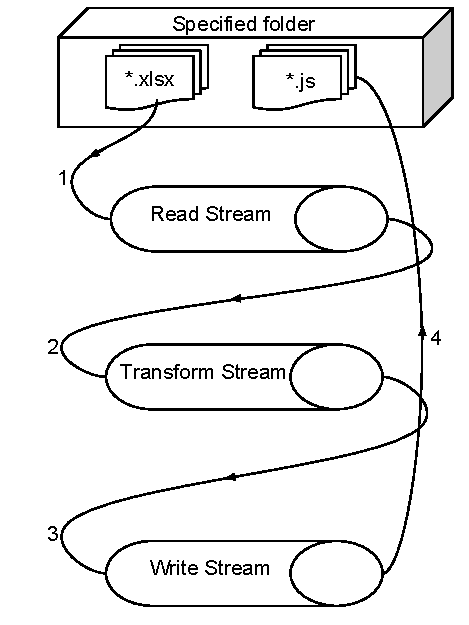
\includegraphics[scale=0.75]{grafiken/TSGeneratorArchitecture}
	\caption{Information flow}
\end{figure}

\begin{enumerate}
	\item \textbf{\textit{Read Stream}} accepts directory address and \textit{pulls} content of all spread sheet files together with their metadata  from this directory including nested directories. From this stream perspective the \textit{Transform Stream} will be referred as an \textit{up stream};
	\item \textbf{\textit{Transform Stream}} accepts the data object with the file name, content, metadata from upstream, creates TestSheet schema and generates content of javascript file implementing \textit{interpreter pattern}. From this stream perspective the \textit{Read Stream} will be referred as an \textit{down stream}, and \textit{Write Stream} as an \textit{up stream}; 
	\item \textbf{\textit{Write Stream}} \textit{pulls} data from upstream. Then is performs an attempt to read the representative .js file from the  specified folder. If the file exists and its last update date is older then for spreadsheet file then the next step will be skipped. If the file does not exist or its the last update date is earlier then the last update date of spreadsheet file then it creates/overwrites javascript file. From this stream perspective the \textit{Transform Stream} will be referred as an \textit{down stream};
\end{enumerate}

As was already described streams are deferred analog of arrays, which allows to perform such operations as mapping, reducing and filtering. The process of transformation of xlsx files to js files in this application is treated as mapping process in general case, and filtering for avoiding of redundant file's overwriting in case if a source xlsx file was not updated.

The folder/file structure of the application looks as following:
\begin{itemize}
	\item index.js
	\item package.json
	\item ReadMe.md
	\item lib/
	\begin{itemize}
		\item scheme/
		\begin{itemize}
			\item index.js
			\item execution\_scheme.js
			\item order.js
			\item scheme.js
		\end{itemize}
		\item stream/
		\begin{itemize}
			\item index.js
			\item read\_stream.js
			\item transform\_stream.js
			\item write\_stream.js
		\end{itemize}
		\item template/
		\begin{itemize}
			\item index.js
		\end{itemize}
	\end{itemize}
	\item test/
	\begin{itemize}
		\item read\_stream.js
		\item write\_stream.js
		\item transform\_stream.js
		\item scheme.js
		\item execution\_scheme.js
		\item order.js
		\item template.js
		\item doublers/
		\begin{itemize}
			\item TestSheetOjbect.js
			\item TestSheet.xlsx
			\item TestSheet.js
		\end{itemize}
	\end{itemize}
	\item node\_modules/
\end{itemize}
%Creation of folders for scheme and template directories is made for purpose of expansion in case of adding Non-linear and/or HigherOrder Test Sheets. 
Each directory unifies node modules for implementation of representative logic. Every folder has \textit{index.js} file which is the public interface file of the module. The default behavior of the \textit{require} method from node.js is to require the \textit{index.js} file from folder if path to it is passed as an input parameter, and file if an input parameter is a path to the file.

The entry point of the system ./index.js looks as following (Listing: \ref{index}):

\lstinputlisting[
language=Javascript, numbers=left, stepnumber=5, firstnumber=1, breaklines=true, 
basicstyle=\footnotesize,
numberstyle=\tiny,
caption={index.js},
captionpos=b,
label=index
]
{code/index.js.txt}

The program invoked from the command line interface accepts one parameter - path to the folder with xlsx files which stores Test Sheets defined by users. The \textit{argv} property of \textit{process} is an array of parameters with which the node module was called from a command line interface. The first parameter is a module name. All next parameters are the arguments passed to this module.




\chapter{Design Principles}
\label{chap:design}
The implementation of each part of the system was made with application of Test Driven Development.The testing framework is \textit{mocha} \url{https://mochajs.org/}. For the creation of doublers (mocks, stubs and spies) for object and method was used \textit{sinon.js }\url{http://sinonjs.org/}.

Application of Test Driven Development principles provide better control over the system on a code level but not on design. In the same time Robert Martin \cite{MartinASD} defined symptoms of not agile design as following:
\begin{itemize}
	\item Rigidity - The design is difficult to change;
	\item Fragility - The design is easy to break;
	\item Immobility - The design is difficult to reuse;
	\item Viscosity - It is difficult to do the right thing;
	\item Needless complexity - Overdesign;
	\item Needless repetition - Mouse abuse;
	\item Opacity - Disorganized expression;
\end{itemize}


To avoid creation of such software John Dooley \cite{Dooley} and Rober Maritn \cite{MartinASD} suggested the following principles of agile architecture:
\begin{itemize}
	\item Closing - Encapsulate things in your design that are likely to change.
	\item Code to an Interface - rather then to an implementation. 
	\item Do not repeat yourself - Avoid the duplication of the code.
	\item The Single-Responsibility Principle - A class should has the only one reason to change from the business perspective;
	\item The Open/Closed Principle - Software entities (classes, modules, functions, etc.) should be open for the extension but closed for modification
	\item The Liskov Substitution Principle - Subtypes must be substitutable for their base types.
	\item The Dependency-Inversion Principle - 		
	\begin{itemize}
		\item High-level modules should not depend on low-level modules.  Both should depend on abstractions. 
		\item Abstractions should not depend upon details. Details should depend upon abstractions.
	\end{itemize}
	\item The Interface Segregation Principle - Clients should not be forced to depend on methods they do not use.
	\item Principles of Least Knowledge - Talk to your immediate friends. 
	\item Principle of Loose Coupling - object that interact should be loosely coupled with well-defined intefaces.
\end{itemize}

This principles are suggestional and can not be strictly followed due to their mutually exclusive nature.

\chapter{Conventions}
\label{sec:convnetions}
Following conventions were developed with respect to the requirements defined by figo GmbH and must be followed by Test Sheet for proper work of developed system:
\begin{itemize}
	\item Number of columns within one Test Sheet should not exceed 26 columns (from A to Z);
	\begin{itemize}
		\item \textbf{A1} cell - description of the test case;
		\item \textbf{A2} cell - module under test (folder with index.js or file with js extension);
		\item \textbf{A3..n} cells - name of the class/object under the test;
		\item \textbf{B3..n} cells - name of the method from representative class/object under the test;
		\item \textbf{C2..n} cells to \textbf{Invocation Column}   - input parameters for representative method under the test;
	\end{itemize}
	\item Invocation delimiters must be allocated within the single column (aligned to the longest row);
	\begin{itemize}
		\item \textbf{Invocation Column} - the column for separation of input values from expected output value(s) filled with $|$ (pipe)(for comparison by scheme and data types) $||$ (two pipes)(for deep comparison - by scheme, data types and values) as a cells values until the last line which includes objects under tests;
	\end{itemize}
	\item \textbf{Expected Return} - column must be next after invocation line.
	\item All functions under test should be asynchronous and accept callback as a last input parameter with standard signature for handling emitted event;
	\item References to the columns with expected return values will accept as value the value obtained from the method execution;
	\item References must be defined only to cells in one of the previous rows;
	\item Files extensions must be xlsx.
\end{itemize}

\chapter{Implementation}
\label{chap:implementation}
For the description of data structures processed by the system, we will use following module (Listing: \ref{demo}) which implements a stack with asynchronous methods (respond time for each method is delayed 10 milliseconds). Usage of the \textit{setTimeout()} method guarantees its asynchronism. While the fact that the timeframe for the response is hard coded into scraping scripts ensures that this method is valid for usage as a proof of concept within the current research topic.
\lstinputlisting[
language=Javascript, numbers=left, stepnumber=5, firstnumber=1, breaklines=true, 
basicstyle=\footnotesize,
numberstyle=\tiny,
caption={stack.js},
captionpos=b,
label=demo
]
{code/demo/stack.js.txt}
The Test Sheet for test coverage of this module looks as following (Figure: \ref{fig:demoTS}). Note that this test coverage was made for the  purpose to show handling of asynchronous testing of real-time software but not to cover the stack module. There are both types of comparison in invocation lines (Column \textbf{D}). The red arrows indicate the references withing this test sheet.
\begin{figure}[H]
\centering
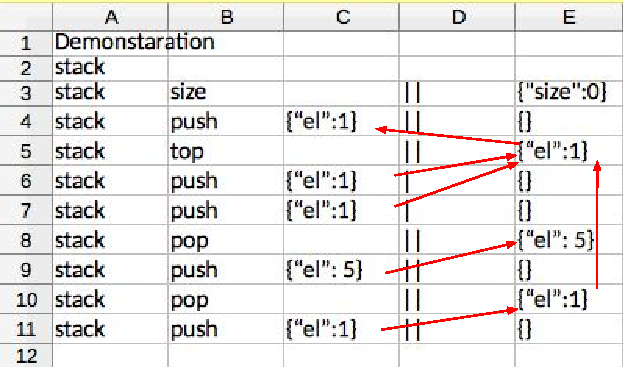
\includegraphics[width=\linewidth]{grafiken/demoTS.pdf}
\caption{Test Sheet coverage for stack.js}
\label{fig:demoTS}
\end{figure}


For the reading of the content from the spread sheet and transforming obtained information into javascript code with further writing of it into a js file the system uses following dependencies upon external npm packages:
\begin{itemize}
	\item Development dependencies:
	\begin{itemize}
		\item  "fs-readdir": "0.0.3", (\url{https://www.npmjs.com/package/fs-readdir});
		\item "through2": "2.0.0", (\url{https://www.npmjs.com/package/through2});
		\item "xlsx": "0.8.0", (\url{https://www.npmjs.com/package/xlsx});
		\item "multipipe": "0.3.1", (\url{https://www.npmjs.com/package/multipipe})
	\end{itemize}
	\item Testing dependencies:
	\begin{itemize}
		\item "mocha": "2.3.4", (\url{https://www.npmjs.com/package/mocha})
		\item "sinon": "1.17.2", (\url{https://www.npmjs.com/package/sinon})
	\end{itemize}
\end{itemize}

\section{Read Stream}
\label{sec:read}
This part of the system is an implementation of combining streams pattern. From the internal view, it consists of two streams.  The first stream is implemented with the use  \textbf{getFilesStream} function from\textbf{ fs-readdir} module. It creates readable stream for reading content of directory including nested directories and returns the array with absolute paths to them.
Second stream is \textbf{getDataStream} the stream in an object mode. For every file path, it accepts from the down stream, it checks its extensions and if it is equal to \textit{.xlsx} this stream implements the reading content of files. For this purpose it uses \textbf{xlsx} module. While for reading files' metadata the internal node.js module \textbf{fs}is used. Next, this stream pushes obtained data to the up stream (Listing: \ref{readStream}).
 
\lstinputlisting[
language=Javascript, numbers=left, stepnumber=5, firstnumber=1, breaklines=true, 
basicstyle=\footnotesize,
numberstyle=\tiny,
caption={read\_stream.js},
captionpos=b,
label=readStream
]
{code/lib/stream/readStream.js.txt}

These two streams are piped into combined stream using module \textbf{multipipe} and returned by the function exported by this module.
In other words, this module exports function which accepts path to the directory and returns array of deferred values to the upstream. Each of deferred value  is a javascript object with following structure (Listing \ref{readOut})
\lstinputlisting[
language=Javascript, numbers=left, stepnumber=5, firstnumber=1, breaklines=true, 
basicstyle=\footnotesize,
numberstyle=\tiny,
caption={Read Stream Output  / Transform Stream Input JSON},
captionpos=b,
label=readOut
]
{code/readOut.js.txt}

\subsection{Test Coverage}
Following test cases show step every incrementally performed during the development process. All calls to systems I/O (e. g. read file meta data, read file) are implemented using stubs. \textbf{Stub} is an implementation of \textit{proxy pattern} which allows to redefine functions behavior. This gives an opportunity to improve speed of tests by replacing functions with call to I/O with empty functions.
%\lstinputlisting[
%language=Javascript, numbers=left, stepnumber=5, firstnumber=1, breaklines=true, 
%basicstyle=\footnotesize,
%numberstyle=\tiny,
%caption={Test coverage for read\_stream.js},
%captionpos=b,
%label=readTest
%]
%{code/test/readStream.js.txt}

The result of tests execution  for this module is following (Fig.: \ref{fig:testRead}):
\begin{figure}[H]
	\centering
	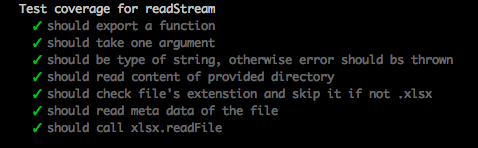
\includegraphics[width=\linewidth]{grafiken/testReadStream.png}
	\caption{Test coverage for read\_stream.js}
	\label{fig:testRead}
\end{figure}



\subsection{Correspondence to the design principles}
\begin{itemize}
	\item Closing - the part of the code responsible for the reading content of the file with the concrete extension and the concrete structure is encapsulated with \textit{getDataStream} function
	\item Code to an Interface - no references to any classes;%the communication is done via standard stream interface.
	\item Do not repeat yourself - no code duplication;
	\item The Single-Responsibility Principle - % can be changed only due to the introduction of new requirements for support multiple sheets within the one xlsx file;
	\item The Open/Closed Principle - functionality of the library can be extended via adding new pipes with application of different piping patterns in a single place;
	\item The Liskov Substitution Principle - object composition is used over inheritance (function wrapped in to pipe object);
	\item The Dependency-Inversion Principle - communication with other modules is done via standard interface.
		\begin{itemize}
			\item Higher level module \textit{index.js} does not depend on implementation current library
			\item Current library depends on the input type provided by the \textit{index.js}
		\end{itemize}
	\item The Interface Segregation Principle - composition over inheritance and usage of standard interfaces;
	\item Principles of Least Knowledge - communication done only with \textit{xlsx} files;
	\item The Principle of Loose Coupling - communication is done via standard file system and standard stream interfaces.
\end{itemize}
%\begin{itemize}
%	\item Closing - stream is closed over file extension, schema\_maker - object structure returned by 	\textit{xlsx} library;
%	\item Code to Interface - stream obtains and returns values via standard stream interface, call to file system made via standard nodeJS File System stream interface;
%	\item Do not Repeat Yourself - no code duplication;
%	\item Single Responsibility Principle - can be changed only due to the change of input type;
%	\item Open Close Principle - new pipes can be added in a single place;
%	\item Liscov Substitution Principle - no inherited objects used;
%	\item Interface Segregation Principle - no dependency on redundant methods;
%	\item Dependency Inversion Principle - higher level module index.js does not depend on current library
%	\item Least Knowledge Principle - communication to interfaces and invocation of used library;
%	\item Loose Coupling Principle - standard interfaces;
%\end{itemize}
%
%\textbf{Design principles implication:}
%\begin{itemize}
%\item  S. - Single Responsibility Principle - can be changed only due to the change of input type
%\item  O. - Open Close Principle - new pipes can be added in a single place
%\item  L. - Liscov Substitution Principle - no inheritance
%\item  I. - Interface Segregation Principle - Stream interface / File System interface
%\item  D. - Dependency Inversion Principle - Higgher level module index.js does not depend on current library
%
%Writer structure:\\


\section{Transform Stream}
\label{sec:transform}
This part of the system performs translation of the Test Sheet into executable javascript code. From the perspective of this module the translation performed in two stages (Listing: \ref{transformST}) 


\lstinputlisting[
language=Javascript, numbers=left, stepnumber=5, firstnumber=1, breaklines=true, 
basicstyle=\footnotesize,
numberstyle=\tiny,
caption={transform\_stream.js},
captionpos=b,
label=transformST
]
{code/lib/stream/transformStream.js.txt}

The\textbf{ first stage} is a creation of \textit{scheme} object of the Test Sheet. The \textbf{second stage} is an application of a template to the content of Test Sheet and the execution schema which has been created on a previous stage. The result of this transformation is pulled by the upstream as a \textit{content} property of an object together with \textit{meta data} and \textit{fileName} obtained from the downstream (Listing: \ref{writeIn}).

\lstinputlisting[
language=Javascript, numbers=left, stepnumber=5, firstnumber=1, breaklines=true, 
basicstyle=\footnotesize,
numberstyle=\tiny,
caption={Transform Stream Output / Write Stream Input JSON},
captionpos=b,
label=writeIn
]
{code/writeIn.js.txt}

\subsection{Test Coverage}
Following test cases can show every step incrementally performed during the development process. Including invocations of helper methods from \textit{scheme} and \textit{template} modules.
%\lstinputlisting[
%language=Javascript, numbers=left, stepnumber=5, firstnumber=1, breaklines=true, 
%basicstyle=\footnotesize,
%numberstyle=\tiny,
%caption={Test coverage for transform\_stream.js },
%captionpos=b,
%label=writeIn
%]
%{code/lib/stream/transformStream.js.txt}

The result of test execution:
\begin{figure}[H]
	\centering
	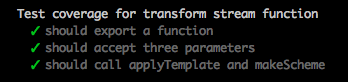
\includegraphics[width=\linewidth]{grafiken/testTransform.png}
	\caption{Test coverage for transform\_stream.js}
	\label{fig:testTransofm}
\end{figure}

\subsection{Correspondence to the design principles}
\begin{itemize}
	\item Closing - the creation of data structure to be transformed to the next stream is created in a single function;
	\item Code to an Interface - this module does not refer to any class. 
	\item Do not repeat yourself - no code duplication;
	\item The Single-Responsibility Principle - can be changed only due to the change of Test Sheet type (another type of scheme);
	\item The Open/Closed Principle - new pipes can be added in a single place with adding new functions to be wrapped in them;
	\item The Liskov Substitution Principle - object composition over inheritance (function wrapped in to pipe object);
	\item The Dependency-Inversion Principle - 
				\begin{itemize}
					\item Higher level module \textit{index.js} does not depend on implementation current library;
					\item Current library depends on the input object provided by the previous stream;
				\end{itemize}
	\item The Interface Segregation Principle -  does not depend on methods since it only creates data object to be passed to the next stream;
	\item Principles of Least Knowledge - direct communication done only with helper functions for schema creation and content generation. 
	\item The Principle of Loose Coupling - communication is done via the standard stream interface
\end{itemize}


\section{Scheme}
\label{sec:scheme}
This part of the system creates a scheme object from the Test Sheet, the only parameter accepted by the main function of this module is a Test Sheet object (the content of xlsx file in a JSON format).
%The decision to perform scheme creation in two stages was made due to the structure of the input object.

The \textbf{first stage} is creation of the object with following properties:
\begin{enumerate}
	\item description;
	\item moduleUnderTest;
	\item objectsUnderTest;
	\item methodsUnderTest;
	\item inputs;
	\item invocations;
	\item outputs;
\end{enumerate}

 The values of each property except \textit{description} and \textit{moduleUnderTest} are arrays of strings with values which represent cell addresses for representative property of the Test Sheet. For the first two properties the values are strings with data  from the cells \textit{A1} and \textit{A2} respectively(Listing: \ref{firstScheme}).

\lstinputlisting[
language=Javascript, numbers=left, stepnumber=5, firstnumber=1, breaklines=true, 
basicstyle=\footnotesize,
numberstyle=\tiny,
caption={Result of the first stage of Test Sheet scheme creation},
captionpos=b,
label=firstScheme
]
{code/firstSchema.js.txt}

The \textbf{sectod stage} is a pivot transformation of the scheme provided from the previous stage. The output of this transformation is an object with properties as a numbers of rows in the Test Sheet object. The values for first and second properties are values of \textit{description} and \textit{module} under test from the respective Test Sheet. While next of them are objects which consist of following Test Sheet properties: \textit{objectUnderTest, methodUnderTest, inputs, outputs, invocations}. With values as single element arrays with coordinate of respective cell (Listing \ref{scheme}).
\lstinputlisting[
language=Javascript, numbers=left, stepnumber=5, firstnumber=1, breaklines=true, 
basicstyle=\footnotesize,
numberstyle=\tiny,
caption={Result of the scheme creation  for Test Sheet},
captionpos=b,
label=scheme
]
{code/scheme.js.txt}

%\lstinputlisting[
%language=Javascript, numbers=left, stepnumber=5, firstnumber=1, breaklines=true, 
%basicstyle=\footnotesize,
%numberstyle=\tiny,
%caption={Module for creation of the Test Sheet scheme},
%captionpos=b,
%label=writeIn
%]
%{code/lib/scheme/index.js.txt}
\subsection{Test Coverage}
Following test cases can show every step incrementally performed during the development process. Since the object obtained from the reading of xlsx file is passed from one part of the system to another (\textit{Object pool OOP pattern}) this module does not perform any I/O calls. There are getter function for each type of cell in a Test Sheet as well as pivot function called \textit{transformScheme} and helper for it called \textit{getRowFromField}.
%\lstinputlisting[
%language=Javascript, numbers=left, stepnumber=5, firstnumber=1, breaklines=true, 
%basicstyle=\footnotesize,
%numberstyle=\tiny,
%caption={Test coverage for creation of the Test Sheet scheme},
%captionpos=b,
%label=writeIn
%]
%{code/test/scheme.js.txt}

The result of test execution:
\begin{figure}[H]
	\centering
	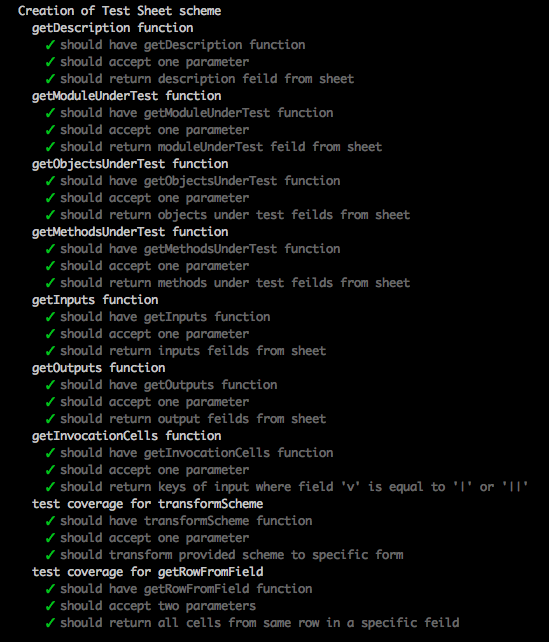
\includegraphics[width=\linewidth]{grafiken/testScheme.png}
	\caption{Test coverage for scheme.js}
	\label{fig:testScheme}
\end{figure}

\subsection{Correspondence to the  design principles}
\begin{itemize}
	\item Closing - comparison type is closed within the \textit{getInvocationCells} function, all elements of Test Sheet are obtained via separate getter functions;
	\item Code to an Interface - all methods have the same minimal abstraction layer for object which represents the content of Test Sheet. All keys of the object should be named as a two dimensional addresses of the cells (i. e. \textit{A1}, \textit{D7} etc);
	\item Do not repeat yourself - no code repetition.
	\item The Single-Responsibility Principle - \textit{transformScheme} function should be changed in case of introduction of the non-linear Test Sheets, since this type has behavior definition in rows under test steps;
	\item The Open/Closed Principle - violated in a \textit{transformScheme} function;
	\item The Liskov Substitution Principle - no inheritance.
	\item The Dependency-Inversion Principle - does not have any lower level modules;
	\item The Interface Segregation Principle - does not have any lower level modules;
	\item Principles of Least Knowledge - can be invoked only via direct import;
	\item The Principle of Loose Coupling - exports single function;
\end{itemize}

\section{Execution Order}
\label{sec:execOrder}
This part of the system is responsible for the definition of an order for the test steps execution. It is called in the main entry point of the scheme module and applied to the pivoted scheme described above and the sheet object the scheme relates to. In a general case, the execution order of tests for a Basic Test Sheet is defined by the order of test steps.
All Test Sheets support references it provides an ability to define input for one test step as an output of some of the previous steps.


However, in \textit{asynchronous} software the moment when execution is completed comes after the period of time when the next function can invoked. Moreover, \textit{real-time} systems have time constraints on their execution, but do not provide an exact time within it will be completed. Further, due to the requirements for the generated tests proposed by figo GmbH test execution should be fast since it will be performed in a timely fashion. Combination of this factors forced to define moment of each test step execution with respect to the source of their input parameters.


For the definition of test steps execution order the decision was taken is to separate test steps in two types. \textit{The first} type covers test steps which behavior does not make influence to the next steps (do not define input parameters for further test steps) and is not determined by any of previous test steps. \textit{The second} type covers test steps which execution result determines behavior of the next test steps or is defined by previous steps.

%
% But the fact that in this case Basic Test Sheets are applied  for \textit{asynchronous} testing of \textit{real-time} software together with an ability to 
%This shit is important for application for real time software.
The process of order definition is following. Main function accepts two input parameters: \textit{sheet} - the content of xlsx file which defines the Test Sheet and \textit{scheme} - the object generated by the main function from \textit{scheme.js} file (Listing: \ref{order}). Walking through the scheme elements starting with the third (skipping service rows) performs the check for each cell in a sheet object for determining does behavior of test step define inputs of any next test step. In this case such test step will be pushed to the \textit{chain} array as the first element and all dependent test steps will be pushed to the nested array as a list of dependent test steps. If \textit{chain} is not empty it will be pushed to the global (in a function scope) \textit{chains}  array. All other rows will be pushed to the \textit{linear array}.


\lstinputlisting[
language=Javascript, numbers=left, stepnumber=5, firstnumber=1, breaklines=true, 
basicstyle=\footnotesize,
numberstyle=\tiny,
caption={Generation of tree structure as a list of childnodes},
captionpos=b,
label=order
]
{code/order.js.txt}

For the further creation of test steps execution order the list of child nodes should be merged into nested list for child nodes which has other child nodes. In terms of test steps this means that the result one test step can define the behavior of few next steps either directly or via some intermediate test steps. 
The merging process is performed by the \textit{transformation} function (Listing \ref{transformation}). It accepts an array object (\textit{chains} array described previously) and performs iterative walk through with recursive call for each nested array. During each iteration this function checks the values of childes (nested arrays) for each of them being a parent for other child nodes (is it present as a first element in next arrays). In such case it takes list of its child nodes and creates a two dimensional array which replaces the the parent element in a list of childes with removing parent entry together with its child nodes from the current position. This operation of replacement performed recursively through all nested arrays using \textit{isIn} function which determines if given element belongs to the provided array including nested arrays.

\lstinputlisting[
language=Javascript, numbers=left, stepnumber=5, firstnumber=1, breaklines=true, 
basicstyle=\footnotesize,
numberstyle=\tiny,
caption={Generation of nested data structure},
captionpos=b,
label=transformation
]
{code/transformFunction.js.txt}

The final step is the  concatenation of arrays from the \textit{first} and the \textit{second} test steps types. In this example, rows \textit{one} and \textit{two} belong to the first type as a service rows which do not define any test steps together with rows \textit{three} and \textit{four}. Note that the input parameter for the test step defined in a row number four is referenced by the expected output of the test step that was defined in a row five. However, the input parameter can not be changed by the execution process of test step and can be passed to the next step before the execution starts without any logic violation. At the same time result of test step \textit{five} is an input parameter for the steps \textit{six}, \textit{seven} and \textit{ten} this in turn defines an input for the test step \textit{eleven} (Listing: \ref{orderSteps}).
\lstinputlisting[
language=Javascript, numbers=left, stepnumber=5, firstnumber=1, breaklines=true, 
basicstyle=\footnotesize,
numberstyle=\tiny,
caption={Execution order},
captionpos=b,
label=orderSteps
]
{code/executionOrderSchema.js.txt}


\subsection{Test coverage}

The following test cases can show every step incrementally performed during the development process. Here you also can see application of Object pool pattern which helped to get rid of the call to I/O for the process of reading content from the .xlsx file.
\begin{figure}[H]
	\centering
	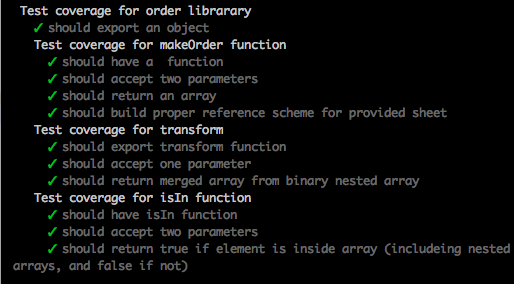
\includegraphics[width=\linewidth]{grafiken/testOrder.png}
	\caption{Test coverage for order.js}
	\label{fig:testOrder}
\end{figure}

\subsection{Correspondence to  the design principles}
\begin{itemize}
	\item Closing - nothing is likely to change;
	\item Code to an Interface - exports a single function;
	\item Do not repeat yourself - no code duplication;
	\item The Single-Responsibility Principle - can be changed only because of the introduction of new types of the Test Sheets;
	\item The Open/Closed Principle - no reason to change, no need for a new functionality;
	\item The Liskov Substitution Principle - no inheritance;
	\item The Dependency-Inversion Principle - does not have any lower level modules;
	\item The Interface Segregation Principle - does not have any lower level modules;
	\item Principles of Least Knowledge -  can be invoked only via direct import;
	\item The Principle of Loose Coupling - exports a single function.
\end{itemize}

\section{Execution Scheme}
\label{sec:execScheme}
This step performs the recursive replacement of elements in an \textit{execution order} array with the elements from the \textit{scheme} object. The function (Listing: \ref{execScheme}) accepts two arguments: \textit{scheme} object and \textit{order} array. If an element is of an input array is an array it then performs recursive call.

\lstinputlisting[
language=Javascript, numbers=left, stepnumber=5, firstnumber=1, breaklines=true, 
basicstyle=\footnotesize,
numberstyle=\tiny,
caption={Application of execution order to the scheme},
captionpos=b,
label=execScheme
]
{code/executionSchema.js.txt}
\subsection{Test Coverage}
Following test cases can show each step incrementally performed during the development process.
\begin{figure}[H]
	\centering
	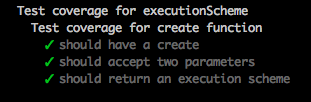
\includegraphics[width=\linewidth]{grafiken/testCreate.png}
	\caption{Test coverage for creation of execution scheme}
	\label{fig:testCreate}
\end{figure}

\subsection{Correspondence to the design principles}
\begin{itemize}
	\item Closing - nothing is likely to change;
	\item Code to an Interface - exports a single function;
	\item Do not repeat yourself - no code duplication;
	\item The Single-Responsibility Principle - nothing is likely to change;
	\item The Open/Closed Principle - no reason to add/change the functionality;
	\item The Liskov Substitution Principle - no inheritance;
	\item The Dependency-Inversion Principle - does not have any lower level modules;
	\item The Interface Segregation Principle - does not have any lower level modules;
	\item Principles of Least Knowledge -  can be invoked only via direct import;
	\item The Principle of Loose Coupling - exports a single function.
\end{itemize}

\section{Template}
\label{sec:template}
The translation to executable javascript file is made by the application of the \textit{template} function. This function accepts three parameters \textit{sheet $<$Object$>$, scheme $<$Object$>$, fileName$<$String$>$}. \textit{Sheet} is a javascript object returned by reading the content of Test Sheet file. The \textit{scheme} is an execution order scheme. The \textit{fileName} is a path to the TestSheet file. This function creates a string content for javascript file based on provided parameters. This function also make indentation and formating of generated file content. The creation takes part in a four stages. 


The \textbf{first stage} is adding a description from the first element of the scheme object. It is enclosed within the multiline comment symbols.


The \textbf{second stage} is adding require of reporting module for representation of execution of the tests result.


The \textbf{third stage} is adding declarations of the module scope variables. The variable names are taken from the coordinates of cells which store input and output parameters in a Test Sheet. The values of the variables are taken from the cells with respective addresses.


The \textbf{fourth stage} is adding calls to the methods (Listing: \ref{applyTemplate}). This stage is the most important part of this module. Since there are two types of execution orders adding function calls is performed in two steps described below. 


The \textit{\textbf{first step}} is adding calls for independent test steps. This is made by iterative call of the \textit{makeCall} function with appending closing brackets to the end of the result string during each of iterations. This function simply performs mapping between \textit{sheet} object (content of xlsx file), \textit{scheme} entry (test step) and string with the content for executable javascript file (Listing: \ref{makeCall}).

\lstinputlisting[
language=Javascript, numbers=left, stepnumber=5, firstnumber=1, breaklines=true, 
basicstyle=\footnotesize,
numberstyle=\tiny,
caption={Function makeCall from template module},
captionpos=b,
label=makeCall
]
{code/makeCall.js.txt}

Note that functions in the generated code are not called directly but via the \textit{call} method of the function's prototype. This method provides an opportunity to call the function from the different context (environment). In the current example the implementation of \textit{stack} module does not depend on the environment in which it was called. But in some cases the result of function's invocation can depend on the environment in which it was invoked. One of such cases can be the creation of child process. The environment for such calls should be passed as an \textit{object under test}.


The \textit{\textbf{second step}} is adding calls for interdependent test steps. For every  element of the \textit{nestedCalls} array it calls the  \textit{makeNestedCall} function and if the next element is an array then this function performs recursive call with an appending of the closing brackets to the result of this call. In case if next element is not an array the it appends closing brackets and performs next iteration (Listing: {\ref{applyTemplate}).



\lstinputlisting[
language=Javascript, numbers=left, stepnumber=5, firstnumber=1, breaklines=true, 
basicstyle=\footnotesize,
numberstyle=\tiny,
caption={Function applyTemplate from template module},
captionpos=b,
label=applyTemplate
]
{code/apply_template.js.txt}


%
%It is implemented as \textit{addCalls} function. This is recursive function which accepts four parameter: \textit{sheet, scheme, indentation, accumulator, fileName}. First two parameters are necessary to access the values represented in a Test Sheet. Next parameter is an indentation level which represents the deepness of a function call by adding representative amount of spaces for each line of generated code. Accumulator parameter is a string to which will be appended result of each recursive call of the function. The last parameter is necessary for report mechanism which allows to record result of the test execution to appropriate file. The report mechanism (e.g \textit{makeComparisonAndWriteResult}) will be described in details within  the next section. However it is important to mention here how it works as a 'black box'. It is binary function which accepts  six parameters. First parameter is an expected return value. Second is an actual returned value received by the callback function, third is a deepness of comparison will be performed for this their values. The function returns \textbf{true} in case of match and after redefinition of the variable takes place. This mechanism allows usage of references within the Test Sheet for asynchronous functions.
%\lstinputlisting[
%language=Javascript, numbers=left, stepnumber=5, firstnumber=1, breaklines=true, 
%basicstyle=\footnotesize,
%numberstyle=\tiny,
%caption={Function addCalls from template module},
%captionpos=b,
%label=template
%]
%{code/lib/template/template.js.txt}


The general case signature for function call generated from this template is following (Listing \ref{gentemplate}):
\lstinputlisting[
language=Javascript, numbers=left, stepnumber=5, firstnumber=1, breaklines=true, 
basicstyle=\footnotesize,
numberstyle=\tiny,
caption={Signature for generated function call},
captionpos=b,
label=gentemplate
]
{code/GeneralTemplate.js.txt}

\subsection{Test Coverage}
Following test cases can show each step incrementally performed during the development process.

%\lstinputlisting[
%language=Javascript, numbers=left, stepnumber=5, firstnumber=1, breaklines=true, 
%basicstyle=\footnotesize,
%numberstyle=\tiny,
%caption={Test coverage for creation of the Test Sheet template},
%captionpos=b,
%label=writeIn
%]
%{code/test/template.js.txt}

The result of test execution:
\begin{figure}[H]
	\centering
	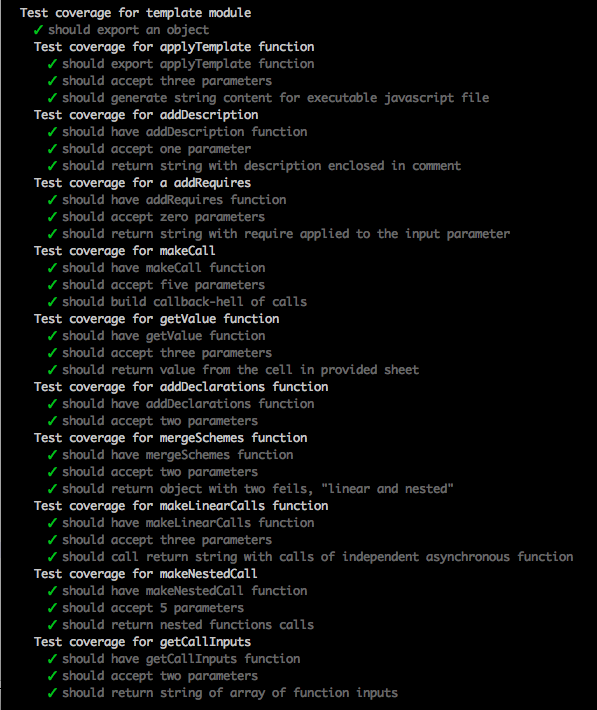
\includegraphics[width=\linewidth]{grafiken/testTemplate.png}
	\caption{Test coverage for template.js}
	\label{fig:testTemplate}
\end{figure}

\subsection{Correspondence to the design principles}
\begin{itemize}
	\item Closing - content generation is enclosed within three independent functions;
	\item Code to an Interface - exports a single function;
	\item Do not repeat yourself - no code duplication;
	\item The Single-Responsibility Principle - can be changed only due to the requirements for generated code;
	\item The Open/Closed Principle - no need to be changed, new functionality can be added via implementation of new version for the \textit{makeCall} function;
	\item The Liskov Substitution Principle - no inheritance;
	\item The Dependency-Inversion Principle - does not have any lower level dependencies;
	\item The Interface Segregation Principle - composition over inheritance;
	\item Principles of Least Knowledge - can be invoked only via direct import;
	\item The Principle of Loose Coupling - exports a single function.
\end{itemize}

e\section{Write Stream}
\label{sec:write}
This part of the system implements on function and exports it wrapped into object stream. It receives an object from the down with the following structure (Listing: \ref{writeIn}). It tries to read meta-data of the file with same name as Test Sheet file but with the .js extension, it is possible only if the file exists. In other case, the exception will be thrown and caught by the \textit{ catch} block which implements the creation of the file with the content received from the down stream. If the file is already exists then the function will be able to read its meta-data. After it, this meta-data will be compared with meta-data of the Test Sheet file received from the down stream. In case if the modification date of the Test Sheet file is bigger then the modification data of the  .js file then the system will overwrite the content of the javascript file with the content that was received from the down stream. In case when the Tests Sheet file was not updated after the creation of the representative js file the system will switch to the next object received from the upstream. The result javascript file generated from the provided Test Sheet looks as following (Listing: \ref{demo})

\lstinputlisting[
language=Javascript, numbers=left, stepnumber=5, firstnumber=1, breaklines=true, 
basicstyle=\footnotesize,
numberstyle=\tiny,
caption={Generated javascript file},
captionpos=b,
label=demo
]
{code/demo/demo.js.txt}

%\lstinputlisting[
%language=Javascript, numbers=left, stepnumber=5, firstnumber=1, breaklines=true, 
%basicstyle=\footnotesize,
%numberstyle=\tiny,
%caption={write\_stream.js},
%captionpos=b,
%label=demo
%]
%{code/lib/stream/writeStream.js.txt}

\subsection{Test Coverage}
The following test cases can show each step incrementally performed during the development process. All calls to systems I/O (e. g. read file meta data, read file) are implemented using stubs.
%\lstinputlisting[
%language=Javascript, numbers=left, stepnumber=5, firstnumber=1, breaklines=true, 
%basicstyle=\footnotesize,
%numberstyle=\tiny,
%caption={Test coverage for write\_stream.js},
%captionpos=b,
%label=writeTest
%]
%{code/test/writeStream.js.txt}


The result of tests execution  for this module is following (Fig.: \ref{fig:testWrite}): 
\begin{figure}[H]
	\centering
	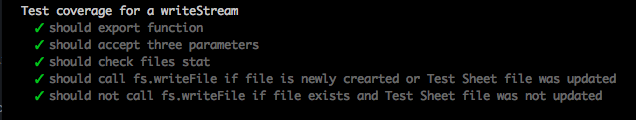
\includegraphics[width=\linewidth]{grafiken/testWriteStream.png}
	\caption{Test coverage for write\_stream.js}
	\label{fig:testWrite}
\end{figure}

\subsection{Correspondence to the design principles}
\begin{itemize}
	\item Closing - module exports the single stream object with the wrapped function.
	\item Code to an Interface - calls are done to the public functions of the required objects. 
	\item Do not repeat yourself - small code duplication in callbacks for file writing, while avoiding this will add more complexity;
	\item The Single-Responsibility Principle - can be changed due to the introduction of requirements for support of multiple sheets within the single xlsx file.
	\item The Open/Closed Principle - performs writing to the file only;
	\item The Liskov Substitution Principle - no inheritance;
	\item The Dependency-Inversion Principle - 
	\begin{itemize}
		\item The Higher level module \textit{index.js} does not depend on implementation current library
		\item Current library depends on the input type provided by the \textit{index.js}
	\end{itemize}
	\item The Interface Segregation Principle - no calls of unnecessary methods;
	\item Principles of Least Knowledge - communication done only with js files;
	\item The Principle of Loose Coupling - communication is done via standard file system and standard stream interfaces.
\end{itemize}

\section{Reporting mechanism}
\label{sec:report}
The reporting mechanism made as a standalone npm package which must be installed globally. This is necessary for an ability to be called by generated javascript files described in a previous section. Since they can be located in different parts of the system. 
The folder/file structure of the application looks as following:
\begin{itemize}
	\item index.js
	\item package.json
	\item ReadMe.md
	\item lib/
	\begin{itemize}
		\item compare\_and\_write.js
	\end{itemize}
	\item test/
	\begin{itemize}
		\item compare\_and\_write.js
	\end{itemize}
	\item node\_modules/
\end{itemize}

\subsection{Implementation}
The system has following dependencies upon external npm packages:
\begin{itemize}
	\item Development dependencies:
	\begin{itemize}
		\item "xlsx": "0.8.0", (\url{https://www.npmjs.com/package/xlsx})
	\end{itemize}
	\item Testing dependencies:
	\begin{itemize}
		\item "mocha": "2.3.4", (\url{https://www.npmjs.com/package/mocha})
		\item "sinon": "1.17.2", (\url{https://www.npmjs.com/package/sinon})
	\end{itemize}
\end{itemize}
	

\lstinputlisting[
language=Javascript, numbers=left, stepnumber=5, firstnumber=1, breaklines=true, 
basicstyle=\footnotesize,
numberstyle=\tiny,
caption={Report mechanism's main function},
captionpos=b,
label=report
]
{code/report.js.txt}

On Figure \ref{fig:resultTestSheet} you see the result Test Sheet created after execution of the generated demo.js file. Note that on line 10 the \textit{pop} method returns value \textit{\{"el": 1 \}} but not the \textit{\{ "el": 5 \}}. This is correct behavior since all the operations are asynchronous and test step 10 does not depend on test step 9. The implementation described in this paper does not guarantee sequential execution of independent test steps. As was already said, this is done for optimization reasons, so that test steps which do not depend upon each other can be started for the execution without waiting for previous step execution being completed. 
\begin{figure}[H]
	\centering
	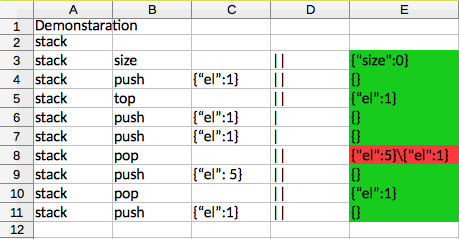
\includegraphics[width=\linewidth]{grafiken/testSheetResult.png}
	\caption{Result Test Sheet for stack.js}
	\label{fig:resultTestSheet}
\end{figure}


\subsection{Test coverage}
The following test cases can show each step incrementally performed during the development process. All calls to systems I/O (e. g. read file meta data, read file) are implemented using stubs.
The result of tests execution  for this module is following (Fig.: \ref{fig:testReport}): 
\begin{figure}[H]
	\centering
	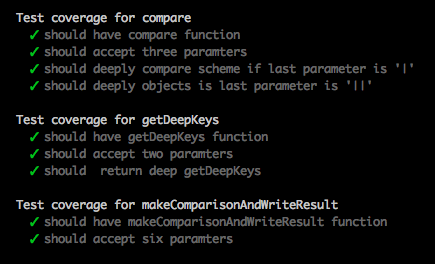
\includegraphics[width=\linewidth]{grafiken/testReport.png}
	\caption{Test coverage for report mechanism}
	\label{fig:testReport}
\end{figure}

\subsection{Correspondence to the  design principles}
\begin{itemize}
	\item Closing - comparison and reporting processes done in the different independent functions;
	\item Code to an Interface - exports a single function;
	\item Do not repeat yourself - no code duplication;
	\item The Single-Responsibility Principle - can be changed only due to the reporting media;
	\item The Open/Closed Principle - new functionality can be added as another exported function;
	\item The Liskov Substitution Principle - no inheritance (required as an npm package);
	\item The Dependency-Inversion Principle - requires standard \textit{assert}, \textit{files system} modules and \textit{xlsx} module;
	\item The Interface Segregation Principle - does not have any lower level modules;
	\item Principles of Least Knowledge -  can be invoked only via the  direct import;
	\item The Principle of Loose Coupling - exports a single function.
\end{itemize}
%\chapter{Test Sheets}
"Software testing is an important aspect of modern software development.
Testing is performed to ensure that a product or component meets the requirements of all stakeholders.
Just as the requirements themselves tests can vary widely in their nature.
Some tests check whether executing certain code paths results in a correct state or answer while others may check whether a certain code path delivers its results in a specified amount of time.

However writing and evaluating tests is often not much different from programming itself.
Tests are usually written in a formal programming language such as Java/JUnit.
This necessitates that in order to create a test and understand its results knowledge of a formal programming language is required.
This is a significant barrier of entry for stakeholders without a background in IT even though they may be interested in the tests themselves.
Even without deep IT knowledge a stakeholder may still be interested in how well a product performs with regard to her requirements.

Visual test representations such as the UML Testing Profile try to lower the barrier of entry into testing.
However most of the time these visualizations are only partial descriptions of the tests and so do not contain all the desired information for evaluation.

The Software Engineering group has started to develop a new representation for tests called Test Sheets.
The goal is to create a way to define tests which combines the power and completeness of formal programming language with a representation that is easy to understand and work with even for people with little IT knowledge.
This is achieved by representing a test in tabular form as a spreadsheet.
Rows in a Test Sheet represent operations being executed while the columns represent input parameters and expected results.
The actual content of a cell can be made dependent on other cells by addressing them via their location.
This works in a way similar to existing spreadsheet software such as Microsoft Excel.
After executing a test the cells for each expected result is colored according to the result of the test.
A successful test causes cells to become green while failed tests are indicated by red cells."\cite{ts}
 \section{Basic Test Sheets}
"A Test Sheet consists of a name and a class being tested. 
Each row after that represents one method call.
The first column identifies the object being tested while the second column indicates which method is being called on said object. [...]
Input parameters are specified in the columns following the method name up to the invocation line. 
Right after the invocation line the expected return values can be specified."\cite{tsb}

% \paragraph{Non-Linear}
%Similar to the invocation line (double line separating input parameters and expected return values) there is a double line below the last method invocation row.
%Below this line the behavior specification starts. 
%Each row of the behavior specification represents a state of a state machine. 
%The state machine starts in the first state that is being specified right below the double line and stops execution once a state is reached without any valid transitions.

%Each column in a row specifies a transition. 
%A transition consists of a guard, executed invocations and a subsequent state. 
%The starting state has only one transition with no guard, the intermediate state has [...] transitions each with a guard and the terminating state does not have any transitions at all[...].  \cite{tsn}

\section{High Order, Parameterized Test Sheets}
"The actual value used for Parameterized Test Sheets is specified by a Higher-Order Test Sheet as in the example below. 
The Higher-Order Test Sheet references the Parameterized Test Sheet as the 'class' being tested. 
On said pseudo-class it invokes the pseudo-method test followed the by the value to be used as parameter. 
?C in the Parameterized Test Sheet is replaced by the value defined the third column (column C) for each execution.
It is also possible to use more than one parameter. These are defined in the Higher-Order Test Sheet in subsequent columns (D, E, F, etc.) and referenced in the Parameterized Test Sheet via ?D, ?E, ?F, etc"\cite{tsh}

%\chapter{NodeJS}
"As an asynchronous event driven framework, Node.js is designed to build scalable network applications. 
Node is similar in design to and influenced by systems like Ruby's Event Machine or Python's Twisted. 
Node takes the event model a bit further, it presents the event loop as a language construct instead of as a library." \cite{nodejsabout}

"Node.js is considered by many as a game-changer—the biggest shift of the decade in web development.[...]\\
 First, Node.js applications are written in JavaScript, the language of the web, the only programming language supported natively by a majority of web browsers. [...]\\
The second revolutionizing factor is its single-threaded, asynchronous architecture. 
Besides obvious advantages from a performance and scalability point of view, this characteristic changed the way developers approach concurrency and parallelism. [...]\\
The last and most important aspect of Node.js lies in its ecosystem: the npm package manager, its constantly growing database of modules, its enthusiastic and helpful community, and most importantly, its very own culture based on simplicity, pragmatism, and extreme modularity. "\cite{nodejsbook}

"JavaScript (JS) is a lightweight, interpreted, programming language with first-class functions. Most well-known as the scripting language for Web pages, many non-browser environments use it such as node.js and Apache CouchDB. JS is a prototype-based, multi-paradigm, dynamic scripting language, supporting object-oriented, imperative, and functional programming styles."\cite{mozillaJS}

\paragraph{Non blocking I/O}
A set of bindings responsible for wrapping and exposing libuv and other low-level functionality to JavaScript.\cite{nodejsbook}

Non blocking I/O in NodeJS is provided by libuv\cite{nodejsabout}\cite{nodejsbook}. 
Which is "libuv is a multi-platform support library with a focus on asynchronous I/O. It was primarily developed for use by Node.js, but it’s also used by Luvit, Julia, pyuv, and others."\cite{libuv}\\
libuv properties\cite{libuvBasic}:
\begin{itemize}
\item Abstract operations, not events
\item Support different nonblocking I/O models
\item Focus on embeddability and perfomace
\end{itemize}


\paragraph{Node core}
A core JavaScript library (called node-core) that implements the high-level Node.js API.

\paragraph{V8/Chakra} the JavaScript engine originally developed by Google for the Chrome browser/ Microsoft for IE 9 browser"\cite{nodejsbook} 

\paragraph{Event handling}
NodeJS asynchronous nature provided by event handler which is an implementation of reactor pattern. Here is the description of process lifecycle\cite{nodejsbook}:
\begin{enumerate}
\item The application generates a new I/O operation by submitting a request to the Event Demultiplexer. The application also specifies a handler, which will be invoked when the operation completes. Submitting a new request to the Event Demultiplexer is a non-blocking call and it immediately returns the control back to the application.
\item When a set of I/O operations completes, the Event Demultiplexer pushes the new events into the Event Queue.
\item At this point, the Event Loop iterates over the items of the Event Queue.
\item For each event, the associated handler is invoked.
\item The handler, which is part of the application code, will give back the control to the Event Loop when its execution completes. However, new asynchronous operations might be requested during the execution of the handler, causing new operations to be inserted in the Event Demultiplexer, before the control is given back to the Event Loop.
\item When all the items in the Event Queue are processed, the loop will block again on the Event Demultiplexer which will then trigger another cycle.
\end{enumerate}

\paragraph{Approaches for asynchronous information flow handling}
\begin{itemize}
	\item \textit{Continuation Passing.} Definition and call of a function within function which performs asynchronous operation
	\item \textit{Callbacks.} Passing as last input parameter function with specific signature for iinput paramteres (error, data), which performs operation/error handling over returned data after it was obtained.
	\item \textit{Async.} JavaScript library which gives an opportunity to write asynchronous functions execution in chain or parallel form within single information flow.
	\item \textit{Promises.} Function can return promise object with can be resolved or rejected in a later time when it particular method will be called by other function.
	\item\textit{Streams.} Piping asynchronous functions one to another. Result of first will be pushed to next stream whenever it is available, or pulled by the next stream whenever it is necessary (depends from stream mode)
	\item\textit{Generators.} Type of constructor introduced in ECMA6 which returns iterator value. Which will iterate through the code unless it will rich yeild method which will wait for return value without blocking event loop.

\end{itemize}

\chapter{Performance}
\label{chap:perfux}
The content of this chapter shows performance measurements made by author regarding Test Sheets processing (generation of executable javascript file from the spreadsheet file) and tests execution.  
All measurements were made on hardware with following characteristics:
\begin{itemize}
	\item Mac mini (Late 2014)
	\item \textbf{Processor:} 2.6 GHz Intel Core i5;
	\item \textbf{Memory:} 8 GB 1600 MHz DD3;
	\item \textbf{Storage:}  1 TB SATA Disk.
\end{itemize}

The characteristics of the tests' execution environment are following:
\begin{itemize}
\item Operational System:
\begin{itemize}
	\item OS X El Capitan
	\item version 10.11.4
\end{itemize}

\item node.js environment:
\begin{itemize}
	\item node version 4.4.5
	\item npm version 2.15.5
\end{itemize}
\end{itemize}


\section{Generation performance}
In this section we describe the system's performance characteristics for generating executable javascript files from the Test Sheet xlsx files. The performance was measured for two cases: the first case is when all the Test Sheet files are located in a single (root) directory, the second case when root directory contains Test Sheet files and another folder with Test Sheet files and yet another folder.
\paragraph{Single folder} - all files are located within the same (root) directory (Diagram: \ref{fig:gs}).
\begin{itemize}
	\item \textbf{New} - all the files are newly added on the every iteration of the measurement with deletion of all the previously generated javascript files. Thus the number of generated js files is equivalent to the number of files in a directory.
	\item \textbf{Add} - only ten xlsx files are added on every iteration of the measurement processes. Thus previously added xlsx files are skipped for javascript files creation. All generated files are skipped as files with non xlsx extension.
\end{itemize}


\begin{figure}[ht]
	\label{fig:gs}
	\centering
	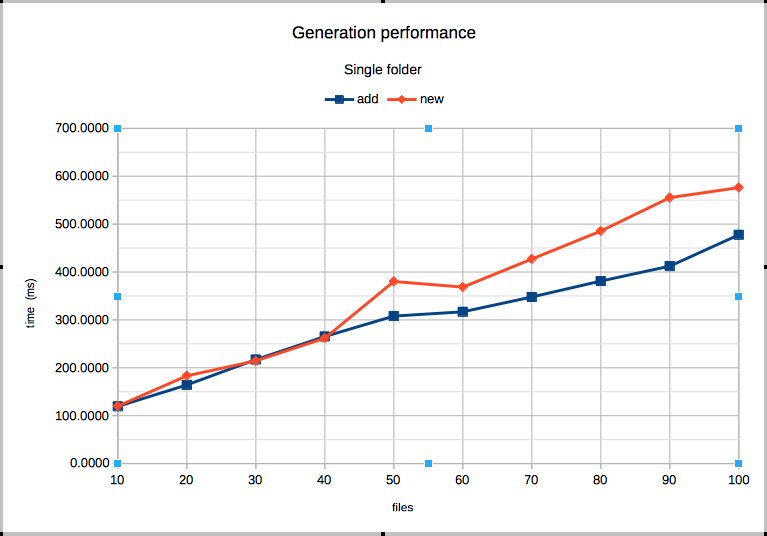
\includegraphics[width=\textwidth]{grafiken/generation_single}
	\caption{Generation performance for files within single folder}
\end{figure}

\paragraph{Nested folder} - each folder contains ten xlsx files and another folder with the same content (Diagram: \ref{fig:gn}).
\begin{itemize}
	\item \textbf{New} - all the files are newly added on the every iteration of the measurement with deletion of previously generated javascript files. Thus the number of created javascript files is equivalent to the number of files in a directory and nested folder(s).
	\item \textbf{Add} - ten xlsx files with the folder nested within the folder created inside the directory from the previous iteration are added. Thus previously added xlsx files are skipped for  the javascript files creation. The javascript files are generated only for the folder with the deepest level of nesting.
\end{itemize}


\begin{figure}[ht]
	\label{fig:gn}
	\centering
	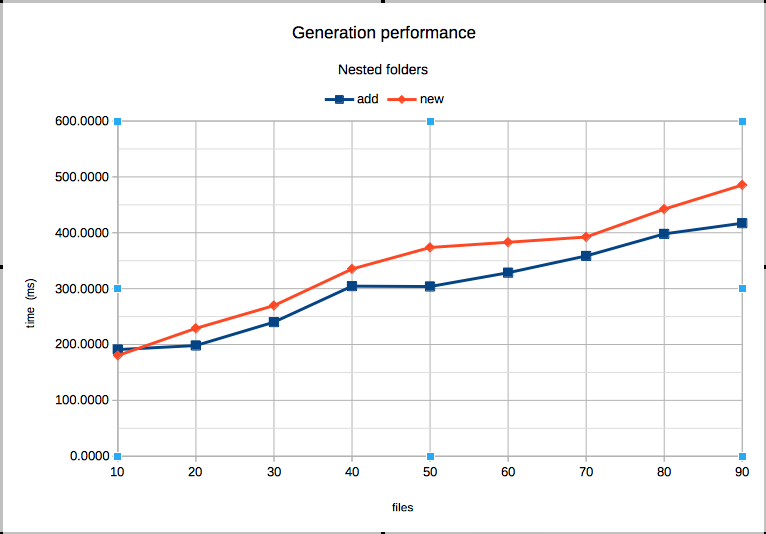
\includegraphics[width=\textwidth]{grafiken/generation_nested}
	\caption{Generation performance for files within nested folders}
\end{figure}

\section{Executions performance}
This section shows execution performance measured for the javascript files generated from the Test Sheet file. All the files are located within the same folder. The measurements were done for two extreme cases of test steps definitions. The first case, when all test step are independent from each other thus can be invoked for execution within the same iteration of the event loop. The second case, when input of all test steps except the first is defined by the result of the previous test step. Thus, there is only one test step called per event loop iteration and the amount of iterations is equal to the number of test steps.
All measurements are done for both deep and scheme only comparisons.

\paragraph{Independent test steps} - all test steps are independent from each other. For this reason their calls are done within the same iteration of an event loop (Diagram: \ref{fig:ei}).
\begin{itemize}
	\item \textbf{Scheme comparison} - actual and expected outputs are compared by their scheme
	\item \textbf{Deep comparison} - actual and expected outputs are compared by their scheme and values of every property
\end{itemize}
\begin{figure}[ht]
	\label{fig:ei}
	\centering
	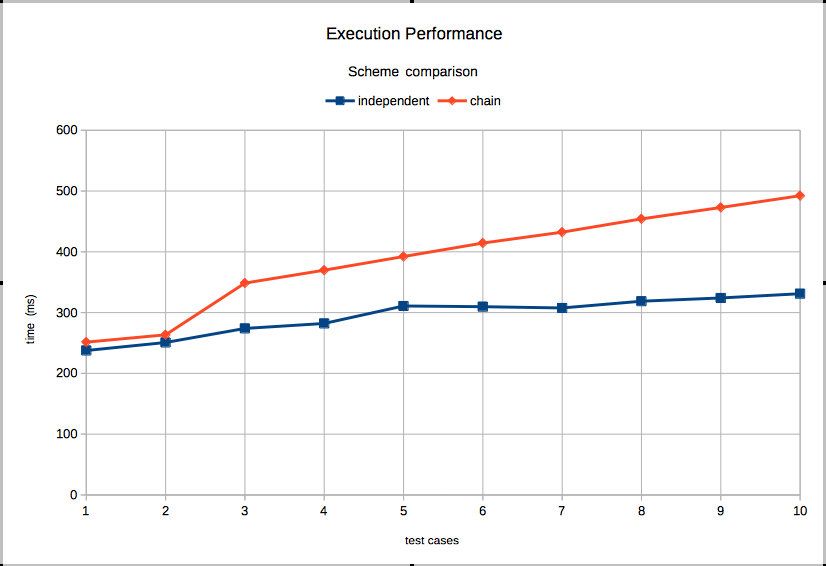
\includegraphics[width=\textwidth]{grafiken/exec_scheme}
	\caption{Execution performance for independent test steps}
\end{figure}

\paragraph{Chain relationship} - output of each test step (except the first) defines input for row below. Therefore there is one execution call per each iteration of the event loop (Diagram: \ref{fig:ef}).
\begin{itemize}
	\item \textbf{Scheme comparison} - actual and expected outputs are compared by their scheme
	\item \textbf{Deep comparison} - actual and expected outputs are compared by their scheme and values of every property
\end{itemize}

\begin{figure}[ht]
	\label{fig:ef}
	\centering
	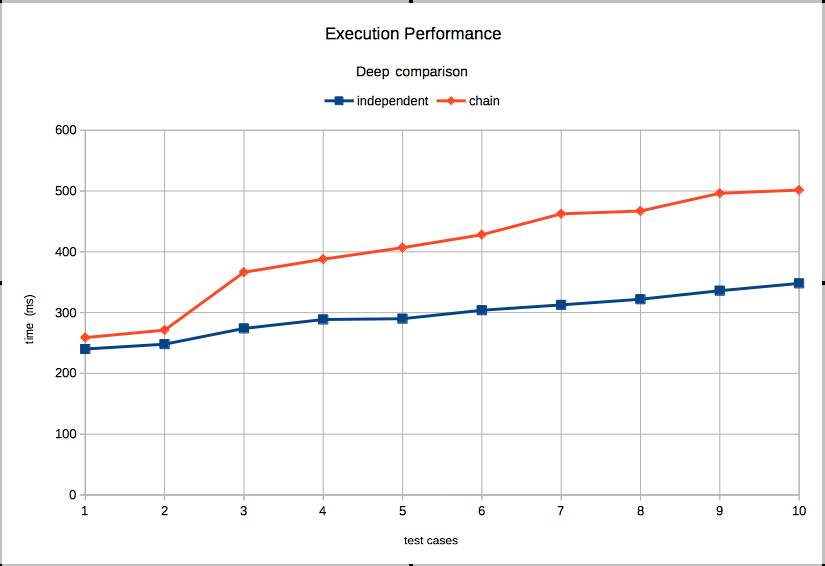
\includegraphics[width=\textwidth]{grafiken/exec_deep}
	\caption{Execution performance for interdependent test steps}
\end{figure}

The measurements from the first section shows that the Test Sheets can be structured within the root folder in arbitrary way without big looses in the generation performance. This should give positive impact on the processes of tests creation and maintenance.

The performance for tests execution proves the necessity of execution order optimization implemented within the \textit{scheme} module. It also shows that type of comparison does not influence the test execution time for small JSON object with simple structure.



\chapter{Limitations and Future Work}
\label{chap:limits}



\begin{enumerate}
	\item for sequential tests execution they should be interdependent $->$ intermediate test steps can be necessary
\end{enumerate}

This paper provide the  prove of concept for usage of Basic Test Sheets only for asynchronous testing of real-time software. The same process can be applied for Higher-Order/Parametrized Test Sheets in a straight forward way since such test sheets just provide additional level of data abstraction without changing generation and execution processes.

However, an application of Non-Linear Test Sheets for such purpose can be non-trivial task due to the finite automates used for definitions of test steps order. In this case, two uncertainties are laying on the surface. First, which event should be taken into account for the calculation of counts the one test step was executed (call event or return event). Second, how to minimize system's time in idle state while it is waiting for response from the external system.

Described implementation requires system under test to have internal logic for handling the execution time. As a future work it is possible to add column for putting additional constraints for execution time of a function under test.

Due to the optimization and nature of asynchronous software some test steps can be started without previous steps being completed which can lead to wrong test assumptions. This can be avoided by making test steps dependent upon previous steps either directly or via additional intermediate test steps.

The implementation  of system described in this paper is bounded to node.js framework, which does not allow to use the  main benefit of javascript language, an ability to be executed inside of the web browser. In such case the browser plug-in for Test Sheets can be developed to work with cloud-based spreadsheet editors. Three changes should be done to make it possible. First is changing the connector library for reading spreadsheet files, same should be done just in case of changing the spreadsheet editor. Next, the  translation software must be compiled to reduce the load on the browser's javascript engine. Furthermore, the compilation has to be done over generated javascript files and they must be recorded into the browser's cache.

All tests are running in a main process. However, in case of figo GmbH each test step creates a child process, this is done automatically as invocation of every script creates child process and Test Sheets are just performing calls to the interface responsible for invocation of the scripts. Further, it is impossible to define time constraints for script execution since they are predefined on the stage of the script development process and are immutable. In case if the script (the child process) does not provide a result withing the specified period of time it will automatically being treated as failed script by the part of the system responsible for its invocation.

Further, all the code covered by tests should be located on the computer where generated javascript files are stored with relative paths to the modules under test. This caused by the fact that node.js' required module works only with relative paths. Moreover system uses standard fs module for I/O operations, but it is the common case to store the code within remote repositories. In combination with the web-browser plug-in it is possible to create the system for remote work with code base from any device which has an Internet connection and able to run web browser which supports javascript.

Last but not least, all asynchronous functions covered by tests implements callback for handling events. This pattern is de facto standard in node.js and creation of promises or stream chunks can be done inside of the callback. However it is possible that the function with asynchronous behavior returns promise object for deferred value, in such case the implementation of template library and reporting mechanism should be changed.

\section{Planned product usage}
Developed prove of concept will be used by figo GmbH in the following use cases.

\paragraph{Internal product management testing tool.} As an original purpose of the Test Sheets.
\paragraph{Automation tool} for customers to automate the routine with the creation of testing data within sandbox environment via implementing calls to API.
\paragraph{Verification tool.} Using Test Sheets employees from business department of the company defines the test steps for verification of the scrapping scripts with the respect to banking web pages. Test files execution is performed as a crown job and automatically executed every five minutes. Verification failure (failed tests) are reported directly to developers.





\chapter{Conclusion}
\label{chap:conclusion}
Proof of concept implemented during this research shows possibility to use Test Sheets concept for asynchronous testing of a real-time software

add some info regarding performance measuments and general impact of an integration of a test sheets in to the enterprise business process






%\chapter{Contributions}
\label{sec:contributions}
For particular implementation of Test Sheets paradigm were developed conventions conventions described below. 
\section{Requirements analysis}
This section describes and analyses requirements differences defined by Test Sheets concept and introduced by figo GmbH.

Test Sheets were originally designed for test definitions of  OOP languages. And all available examples describes tests definitions for Java Classes. While figo GmbH case requires implementation of tests for nodeJS/casperJS, which are based on JavaScript - Object Oriented, imperative, Functional Oriented programming language with asynchronous information flow. Moreover figo GmbH requires input of test results to be recorded in to LogStash logs database. The execution requirements from figo GmbH are such that tests defined via Test Sheets should be automatically executed in a time manner (every 2 mins or so), while normal software testing is performed on demand.
The figo's requirement for comparison is such that while defining a Test Sheet user should be able to select from two types of comparison: 1) Strict comparison - complete comparison of objects including both properties' structure and their values. 2) Not-Strict comparison - scheme comparison of objects.

(Probably should go to different section)
Scraping scripts implement callback based approach for handling asynchronous data flow. This provides an opportunity to perform result comparison within the custom callback defined on a implementation stage.
Standard convention for callback definitions limitates number of input parameters of a callback (error, data), while comparison requires compare data parameter with expected outputs from Test Sheet. The opportunity to resolve this issue lays in a JavaScript's support of functions as a class citizens, the function implementation of module for comparison and report: module exports function which invoked with single parameters (expected\_output) / ( + script name) and returns function which is used as a callback for scrapping script, this callback function performs comparison and writes its result to TestSheet or logstash depending on environment in which the program was executed

\section{Conventions}
\label{sec:conventions}

Following conventions should be followed for Test Sheet passed verification.

\textbf{General:}
\begin{itemize}
\item Number of columns within one TS should not exceed 26 columns (from A to Z);
\item Invocation delimiters must be allocated within single column the (aligned to the longest row);
\item References to the columns with expected returns columns will take as value actual return value obtained from method execution;
\item Files extensions should be .xlsx\\
\end{itemize}

\textbf{ Basic Test Sheets} 
\begin{itemize}
\item A1 cell(optional) - description of the test case;
\item A2 cell - module under testing with an extension (.js);
\item A3..n - name of the class/object under the test;
\item B3..n - name of the method from representative class (same row) under the test;
\item C2..n to Invocation Column - input parameters for representative method (same row) under the test;
\item Invocation Column - the column for separation of input values from expected output value(s) filled with | (pipe)(for comparison by scheme and data types) || (two pipes)(for deep comparison - by scheme, data types and values) as a cells values until the last line which includes objects under tests;
\item Expected Return - column(s) after invocation line.\\
\end{itemize}

%\textbf{ Non-Linear Test Sheets}
%Same convention as for Basic Test Sheets plus following conventions for Behaviour Specification:
%\begin{itemize}
%\item N-th row - the row for separation of test definitions from the test behaiour. Filled with \_ (underscore) until the last column of expect values (excluding invocation column)
%\item N+1-th row - Starting state. Starts with -> following space separated integers which represent testing steps which should be executed first;
%\item N+2-th row - Intermediate state. Each cell of this row should satisfy following syntax requirements: guard ->following space separated integers which represent testing steps which should be executed if condition within guard is true. One of which should be equal to N+3 which represents the final state;
%\item N+3 - Final state. Empty line showing end of testing process.
%\end{itemize}
%Syntax for guard: [\#N <condition> <value | link to the cell>], where:
%\#N - number of times row N has already been executed within current test;
%<condition> - conditional operator (>, >=, <, <=, ==, !=)
%<value | link to the cell> - value or link to the cell with value which should be compared.\\

\textbf{ Parameterized and Higher-Order Test Sheets}
Lower order test sheets can belong to Basic of Non-Linear types of Test Sheets and respectively follow conventions, with next additional option:
\begin{itemize}
\item Input and/or output cells can contain parameters ?[B-Z]+ which represent the value of cells within the representative column of Higher-Order Test Sheet
\item Rows 1 and 2 should follow conventions for Basic Test Sheet;
\item Cells starting from second row inside of [B-Z] columns should contain values which will replace parameters inside of Parameterized Test Sheet.
\end{itemize}

 \section{Use Case}
 definition (possibly in tabular form)


\begin{itemize}
\item Test Sheets defined by users (clients or employees without development background).
\item Tests themselves will be applied for identification of layout changes on a target page before any interaction will appear to avoid errors and minimize the time of scripts correction.
\end{itemize}
 
\textbf{Execution stages:}
\begin{itemize}
\item Automated transformation of Test Sheets into JavaScript tests;
\item Scheduled task for running tests on web pages;
\item Developer notification regarding failing test.
\end{itemize}

The program run by user 
%The implemented program is running as a crown job which is executing JS files generated from xlsx Test Sheets. Each JS file invokes scrapping script via Command Line Interface which in turn performs communication to Bank's web page. Results of script execution are compared with expected outputs from Test Sheet using a callback function. Result of comparison is written to LogStash and original Test Sheet.


\section{Architecture} 
This system implements Pipe-and-Filter Architecture. \cite{Dooley} \cite{nodejsbook}
%with some external complexity included in to piping mechanisms with application of pipeing patterns. 

"In a pipe-and-filter style architecture, the computations components are called filters and they act as transducers that take input, transform it according to one or mode algorithms, and then output the result to communications conduit. The input and outputs coduits are called pipes.\\
The filters must be intedependent components. [...] The clasic example of pipe-and-filter architectural style is the Unix shell[...]"\cite{Dooley}.


\section{Design and Implementation}
Consists of two streams Reader and Writer both streams are in object mode.

The system's information workflow described with following explanatory Test Sheet:\\
\begin{tabular}[h]{| c | l | l | l | l | l | l | }
	\hline
	 \  & A & B & C & D & E & F \\
		\hline
	1 & get Accounts & \ & \ & \ & \ & \ \\
		\hline
	2 & BankAustria & \ & \ & \ & \ & \  \\
		\hline
	3 & BankAustria & login & $<$credentials object$>$ & $<$pin object$>$ & $|$ & \{...\} \\
		\hline
	4 & BankAustria & getAccounts & $<$credentials object$>$ & \ & $||$ & \{...\} \\
	\hline
\end{tabular}

\subsection{Reader}
%Reader accepts directory with Test Sheets (*.xlsx files) as an input parameter and returns a Schema object with a following structure for all directory entries to the standard stream interface.


On a lower level Reader stream consists of two combined streams (streams combination pattern used);

First stream takes input as a directrory and returns list of absolute paths to all files within provided directory (including nested folders);
Second stream accepts output of a first stream and for all .xlsx files obtains its schema invoking function from schema\_maker library and as an output returns object with absolute path to the Test Sheet file with file content returned by reading with object returned by reading file (object pool pattern) with \textit{xlsx} library (\url{https://www.npmjs.com/package/xlsx}) and scheme created by schema\_maker library.\\
\textbf{Schema structure for expample Test Sheet:}
\begin{itemize}
	\item pathToFile: 'absloute/path/to/test/sheet/file';
	\item testsheet: \{ $<$ object returned by xlsx library $>$\};
	\item schema:
		\subitem description: 'get Accounts',
	    \subitem moduleUnderTest: 'BankAustria',
	    \subitem objectsUnderTest: ['A3', 'A4'],
	    \subitem methodsUnderTest: ['B3', 'B4'],
	    \subitem inputs: ['C3', 'C4', 'D3],
    	\subitem outputs: ['F3', 'F4'],
    	\subitem invocations: ['E3', 'E4'],
\end{itemize}

\paragraph{Correspondence to design principles:}
\begin{itemize}
	\item Closing - stream is closed over file extension, schema\_maker - object structure returned by 	\textit{xlsx} library;
	\item Code to Interface - stream obtains and returns values via standard stream interface, call to file system made via standard nodeJS File System stream interface;
	\item Do not Repeat Yourself - no code duplication;
	\item Single Responsibility Principle - can be changed only due to the change of input type;
	\item Open Close Principle - new pipes can be added in a single place;
	\item Liscov Substitution Principle - no inherited objects used;
	\item Interface Segregation Principle - no dependency on redundant methods;
	\item Dependency Inversion Principle - higher level module index.js does not depend on current library
	\item Least Knowledge Principle - communication to interfaces and invocation of used library;
	\item Loose Coupling Principle - standard interfaces;
\end{itemize}

%\textbf{Design principles implication:}
%\begin{itemize}
%\item  S. - Single Responsibility Principle - can be changed only due to the change of input type
%\item  O. - Open Close Principle - new pipes can be added in a single place
%\item  L. - Liscov Substitution Principle - no inheritance
%\item  I. - Interface Segregation Principle - Stream interface / File System interface
%\item  D. - Dependency Inversion Principle - Higgher level module index.js does not depend on current library

%Writer structure:\\

%\end{itemize}
\subsection{Writer}
%\selectlanguage{ngerman} % jetzt sprechen wir deutsch.
%\chapter{Implementierung}

Zusammen mit dem Betreuer werden use-cases entwickelt anhand deren die
Software programmiert werden soll. Diese dienen auch als Bewertungsgrundlage.\\
\\
Die allgemein empfohlene Verzeichnisstruktur eines Projektes sieht wie folgt
aus:

\begin{itemize}
\item projektname
  \begin{itemize}
  \item bin
  \item doc
  \item lib
  \item src
  \end{itemize}
\end{itemize}

Die zu erstellende Software soll im package
de.uni\_mannheim.informatik.swt.\texttt{projektname} unter \texttt{src} liegen.\\
\\
Bei der Programmierung sollte durchgängig die englische Sprache verwendet
werden. Hierzu zählen insbesondere Kommentare im Quellcode, Namen von
Funktionen, Variable, Menüpunkte im Benutzerinterface, kurze
Hilfestellungen und Ausgaben von Programmen.\\
\\
Der Code sollte mit Hilfe von \texttt{lstinputlisting} formatiert und ausgegeben werden, wie in folgendem Beispiel:

\lstinputlisting[
  language=Java, numbers=left, stepnumber=5, firstnumber=1, breaklines=true, 
  basicstyle=\footnotesize,
  numberstyle=\tiny,
  caption={GuestbookForm.java},
  captionpos=b,
  label=GuestbookForm
]
{code/GuestbookForm.java.txt}

%\selectlanguage{english} % jetzt sprechen wir wieder englisch
%\selectlanguage{ngerman} % wenn im Inhaltsverzeichnis Appendix stehen soll, muss Engl gewaehlt sein, fuer Anhang Deutsch
\appendix

%Bibliographie
%waehle einen der folgenden 4 Eintraege
%\bibliographystyle{literatur/natdin} %DIN Style Literaturverzeichnis, comment out pagebackref
%\bibliographystyle{literatur/IEEEtran} % IEEE Style Literaturverzeichnis
%\bibliographystyle{literatur/natdinCustomized} %DIN Style Literaturverzeichnis + Punkt hinter jeder Literaturangabe -> low level config fuer Zitate: natdin.cfg im Projektordner, comment out pagebackref
%\bibliographystyle{literatur/natdinCustomizedEnglish} %DIN Style auf Englisch getrimmt mit Punkt hinter Literaturangabe -> low lovel config fuer Zitate: natdin.cfg im Projektordner, pagebackref kann damit nicht genutzt werden
%\bibliographystyle{aer} % alternativ auch apalike, aer, apalike2... s.a. http://web.reed.edu/cis/Help/LaTeX/bibtexstyles.html
\bibliographystyle{plain} % very nice bib style
%note on aer: does not like inbook entries
%\bibliographystyle{natdin}

\bibliography{literatur/lit} %Pfad zur bib-Datei

%appendices can be defined here, the appendix structure has to be added manually to the toc (table of contents)
%\clearpage  %toc new page
%\addcontentsline{toc}{chapter}{Appendix} %add chapter to toc
\addpart{\appendixname}
%\chapter{First class of appendices}
%\section{Some appendix}
%
%This is a sample appendix entry.

% \newpage
% \input{kapitel/methodologyQuestionMappingTable}
% 
% \input{kapitel/question_origins}
% \include{extern/fragebogenE}
% \include{extern/fragebogenD}
% 
% \input{kapitel/invitationLetters}
% 
% 
% \include{kapitel/coverageTable}

%Eidesstattliche Erklaerung
\chapter*{Eidesstattliche Erkl\"{a}rung}
\thispagestyle{empty}
Hiermit versichere ich, dass diese Abschlussarbeit von mir persönlich verfasst
ist und dass ich keinerlei fremde Hilfe in Anspruch genommen habe. Ebenso
versichere ich, dass diese Arbeit oder Teile daraus weder von mir selbst noch
von anderen als Leistungsnachweise andernorts eingereicht wurden. Wörtliche oder
sinn\-gemäße Übernahmen aus anderen Schriften und Veröffentlichungen in gedruckter
oder elektronischer Form sind gekennzeichnet. Sämtliche Sekundärliteratur und
sonstige Quellen sind nachgewiesen und in der Bibliographie aufgeführt. Das
Glei\-che gilt für graphische Darstellungen und Bilder sowie für alle
Internet-Quellen.

Ich bin ferner damit einverstanden, dass meine Arbeit zum Zwecke eines
Plagiatsabgleichs in elektronischer Form anonymisiert versendet und gespeichert
werden kann. Mir ist bekannt, dass von der Korrektur der Arbeit abgesehen werden
kann, wenn die Erklärung nicht erteilt wird.
\bigskip

\vspace{2.5cm}

Mannheim, \today \hspace{7cm} Unterschrift\\

%Abtretungs Erklaerung
\chapter*{Abtretungserkl\"arung}
\thispagestyle{empty}
Hinsichtlich meiner Studienarbeit/Bachelor-Abschlussarbeit/Diplomarbeit r\"aume ich der Universit\"at Mannheim/Lehrstuhl f{\"u}r Softwaretechnik,
Prof. Dr. Colin Atkinson, umfassende, ausschlie{\ss}liche unbefristete und
unbeschr\"ankte Nutzungsrechte an den entstandenen Arbeitsergebnissen ein.

Die Abtretung umfasst das Recht auf Nutzung der Arbeitsergebnisse in Forschung
und Lehre, das Recht der Vervielf\"altigung, Verbreitung und \"Ubersetzung sowie
das Recht zur Bearbeitung und \"Anderung inklusive Nutzung der dabei
entstehenden Ergebnisse, sowie das Recht zur Weiter\"ubertragung auf Dritte.

Solange von mir erstellte Ergebnisse in der urspr\"unglichen oder in
\"uberarbeiteter Form verwendet werden, werde ich nach Ma{\ss}gabe des Urheberrechts
als Co-Autor namentlich genannt. Eine gewerbliche Nutzung ist von dieser
Abtretung nicht mit umfasst.
\bigskip

\vspace{2.5cm}

Mannheim, \today \hspace{7cm} Unterschrift\\


\end{document}
